% !TeX root = main.tex
% !TEX program = pdflatex

\chapter{Características de los Sistemas de Medida}\label{cap:caracteristicas_sistemas_medida}

En este capítulo se analiza el comportamiento de los sistemas de instrumentación desde dos perspectivas: la \emph{estática}, que describe la relación entrada-salida cuando la magnitud es constante o varía lentamente, y la \emph{dinámica}, que estudia la respuesta temporal y frecuencial ante cambios rápidos de la magnitud física~\cite{bentley2004measurement,pallasareny2000sensors}.


\section{Características Estáticas}\label{sec:caract_estaticas}

Las características estáticas describen el rendimiento de un instrumento cuando la magnitud medida $x$ no varía con el tiempo o lo hace de forma tan lenta que los efectos de inercia o retardos son despreciables. En este régimen, la salida $y$ del sistema se puede modelar como una función de la entrada $x$: $y = f(x)$.

\subsection{Curva de Calibración y Sensibilidad}

La función de transferencia o curva de calibración relaciona la salida $y$ con la entrada $x$: $y = f(x)$. En un sistema ideal, esta relación es lineal: $y = mx + b$, donde $m$ es la pendiente y $b$ el offset u ordenada en el origen del sistema de coordenadas. Sin embargo, en la práctica, los sensores presentan no linealidades, lo que se refleja en una curva de calibración que puede ser polinómica o incluso más compleja.

\begin{itemize}
    \item \emph{Sensibilidad ($S$)}: Es la pendiente de la curva de calibración. 
    \[ S(x) = \frac{dy}{dx} \]
    Si el sistema es lineal, la sensibilidad es constante. En sistemas no lineales (como un termistor NTC, \textit{Negative Temperature Coefficient}), la sensibilidad depende del punto de operación. Por ejemplo, en un termistor NTC, la resistencia disminuye con el aumento de la temperatura, lo que implica que la sensibilidad varía a lo largo del rango de temperaturas. En aplicaciones donde se requiere medir pequeñas variaciones, es crucial seleccionar un sensor con alta sensibilidad en el rango de interés para garantizar una buena resolución y precisión.
    \item \emph{Resolución}: Es el incremento más pequeño de la entrada que produce un cambio perceptible en la salida. En instrumentación digital, suele estar limitada por el número de bits del convertidor analógico digital (\textit{analog to digital converter}, ADC) y el ruido.
\end{itemize}

Esta característica es fundamental para entender la precisión y el rango de operación de un sensor, así como para diseñar sistemas de control que utilicen estas mediciones. Por ejemplo, un sensor con alta sensibilidad puede ser adecuado para medir pequeñas variaciones, pero podría saturarse o ser más susceptible al ruido en rangos más amplios. Por otro lado, un sensor con baja sensibilidad puede ser más robusto frente a perturbaciones, pero podría no ser capaz de detectar cambios sutiles en la magnitud medida. Por ello, la elección del sensor adecuado depende del contexto de aplicación y de los requisitos específicos de medición.

En cuanto a la resolución, es importante considerar que un sistema con alta resolución no garantiza una medición precisa si el ruido es significativo, ya que el ruido puede enmascarar las pequeñas variaciones que el sistema es capaz de detectar. Por ejemplo, en un sistema de adquisición de datos con un ADC de 12 bits y un rango de entrada de 0 a 10 V, la resolución teórica sería de aproximadamente 2.44 mV por bit. Sin embargo, si el ruido del sistema es del orden de varios milivoltios, la resolución efectiva se verá reducida, ya que las pequeñas variaciones en la entrada podrían no ser distinguibles debido al ruido.

\subsection{Error de Cero y Error de Span}\label{sub:error_cero_span}

Una curva de calibración puede ser perfectamente lineal y, aun así, estar equivocada de dos maneras distintas que conviene no confundir, porque no se corrigen igual. Si la recta tiene la pendiente correcta pero está desplazada, el sistema tiene un \emph{error de cero} (o de \emph{offset}): todas las lecturas se desvían la misma cantidad, de modo que el error absoluto es constante y el relativo crece al acercarse al fondo del rango. Si lo que está mal es la pendiente, el error es de \emph{span} o de ganancia: nulo en el punto de referencia y proporcional a la lectura en el resto del rango. Un sistema que presenta ambos defectos responde a
\begin{equation}\label{eq:error_cero_span}
    x_{ind} = (1 + \epsilon_s)\,x + e_0
\end{equation}
donde $e_0$ es el error de cero y $\epsilon_s$ el error relativo de span. La Figura~\ref{fig:errores_cero_span} compara los dos casos con la recta ideal.

\begin{marginfigure}
    \centering
    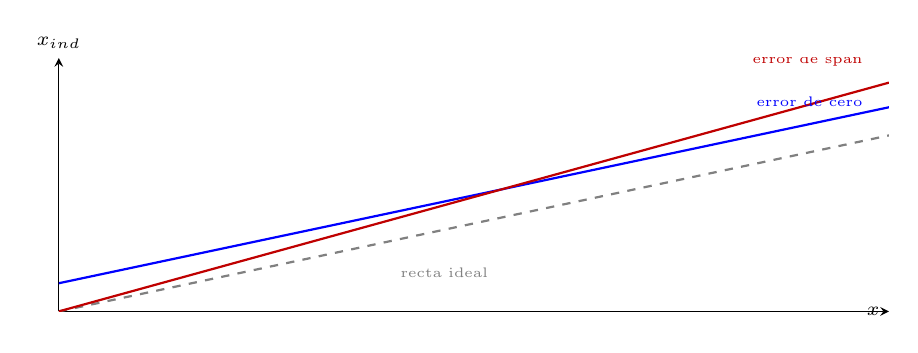
\begin{tikzpicture}
        \begin{axis}[
            width=\linewidth, height=4.8cm,
            xlabel={$x$}, ylabel={$x_{ind}$},
            xmin=0, xmax=5, ymin=0, ymax=7.2,
            axis lines=left, font=\scriptsize,
            xtick=\empty, ytick=\empty,
            every axis y label/.style={at=(current axis.above origin),anchor=south},
            every axis x label/.style={at=(current axis.right of origin),anchor=east},
        ]
            \addplot[gray, dashed, thick, domain=0:5] {x};
            \addplot[blue, thick, domain=0:5] {x+0.8};
            \addplot[red!75!black, thick, domain=0:5] {1.3*x};
            \node[gray, font=\tiny, anchor=north west] at (axis cs:2.0,1.5) {recta ideal};
            \node[blue, font=\tiny, anchor=south east] at (axis cs:4.9,5.55) {error de cero};
            \node[red!75!black, font=\tiny, anchor=south east] at (axis cs:4.9,6.7) {error de span};
        \end{axis}
    \end{tikzpicture}
    \caption[Error de cero y error de span sobre la recta de calibración.]{Los dos defectos de una recta de calibración lineal. El error de cero desplaza la recta entera el mismo valor absoluto --el error relativo es mayor en el fondo del rango--, mientras que el error de span cambia su pendiente y el error crece con la lectura.}\label{fig:errores_cero_span}
\end{marginfigure}

La distinción no es académica: la calibración de un instrumento consiste precisamente en medir esos dos parámetros y corregirlos, ajustando el cero y el span contra un patrón, y por eso el certificado de calibración de cualquier instrumento de laboratorio los declara por separado (Capítulo~\ref{cap:metrologia}). También explica por qué las especificaciones se escriben de dos formas a la vez: los errores de cero se dan en unidades absolutas --milivoltios, grados-- y los de span en tanto por ciento.

\marginnote{\textbf{Ejemplo:} un sensor con un error de span del \SI{0.5}{\percent} sobre un fondo de escala de \SI{100}{\milli\volt} y un error de cero de \SI{1}{\milli\volt}. En el fondo de escala el error combinado es de \SI{1.5}{\milli\volt}, es decir, el \SI{1.5}{\percent} de la lectura; pero a una décima parte del rango, con una lectura de \SI{10}{\milli\volt}, el error sigue siendo de \SI{1.05}{\milli\volt} y ahora representa el \SI{10.5}{\percent} de lo indicado. El error de cero manda en el fondo del rango y el de span, en el extremo superior.}

\subsection{Linealidad y Ajuste por Mínimos Cuadrados}

En ingeniería, siempre preferimos sistemas lineales de la forma $y = mx + b$, ya que facilitan el procesado posterior. Sin embargo, los sensores reales presentan desviaciones. Para obtener la \emph{mejor recta} de ajuste, que se considera la curva de calibración que representa a un sensor en el laboratorio, utilizamos el \emph{Método de los Mínimos Cuadrados}~\cite{taylor1997erroranalysis}, como se muestra en la Figura~\ref{fig:minimos_cuadrados}.
\begin{marginfigure}
    \centering
    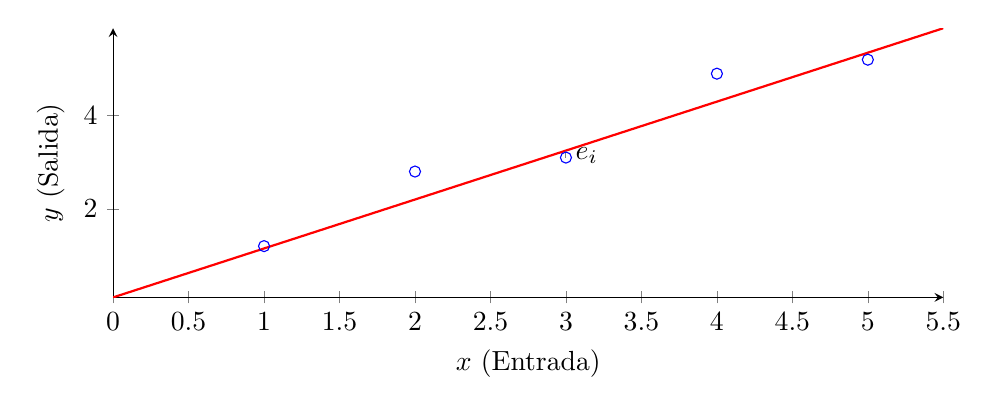
\begin{tikzpicture}
        \begin{axis}[
            width=\linewidth,
            height=5cm,
            xlabel={$x$ (Entrada)},
            ylabel={$y$ (Salida)},
            %font=\small,
            axis lines=left,
            scatter/classes={a={mark=o,draw=blue}},
            legend style={at={(0.5,-0.3)},anchor=north,legend columns=-1}
        ]
            % Puntos experimentales
            \addplot[scatter,only marks,scatter src=explicit symbolic]
                table[meta=label] {
                    x y label
                    1 1.2 a
                    2 2.8 a
                    3 3.1 a
                    4 4.9 a
                    5 5.2 a
                };
            % Recta de ajuste
            \addplot[thick, red, domain=0:5.5] {1.05*x + 0.1};
            
            % Línea de error (ejemplo)
            \draw[dashed, gray] (axis cs:3, 3.1) -- (axis cs:3, 3.25);
            \node[right] at (axis cs:3, 3.15) {$e_i$};
        \end{axis}
    \end{tikzpicture}
    \caption[Ajuste lineal por mínimos cuadrados.]{Ajuste lineal por mínimos cuadrados. La recta minimiza la distancia vertical al cuadrado de cada punto experimental.}\label{fig:minimos_cuadrados}
\end{marginfigure}

Dado un conjunto de $n$ pares de medidas $(x_i, y_i)$, buscamos la recta que minimiza la suma de los cuadrados de los residuos ($e_i$). El residuo para cada punto es la diferencia entre la salida medida $y_i$ y la salida predicha por la recta de ajuste $mx_i + b$:
\[ e_i = y_i - (mx_i + b) \]

El objetivo es encontrar los coeficientes $m$ y $b$ que minimizan la suma de los cuadrados de los residuos:
\begin{equation}\label{eq:error_cuadratico} 
    \sum_{i=1}^n e_i^2 = \sum_{i=1}^n {(y_i - (mx_i + b))}^2 = \sum_{i=1}^n {(y_i - mx_i - b)}^2
\end{equation}

Para obtener la mejor representación lineal de los datos obtenidos en el laboratorio, utilizamos el \emph{Método de los Mínimos Cuadrados}.\marginnote{\emph{Método de los Mínimos Cuadrados $m$ y $b$:}  La demostración de la Ecuación~\ref{eq:m_final} y~\ref{eq:b_final} se basa en la minimización de la función de error cuadrático proporcionada por la Ecuación~\ref{eq:error_cuadratico}, que es la suma de los cuadrados de los residuos. Al derivar esta función con respecto a $m$ y $b$ y establecer las derivadas iguales a cero, se obtienen las fórmulas mencionadas para $m$ y $b$. Este proceso asegura que se encuentra el punto mínimo de la función de error, lo que corresponde a la mejor recta de ajuste para los datos experimentales.

Para minimizar la función de error cuadrático $E(m, b) = \sum_{i=1}^n {(y_i - mx_i - b)}^2$, buscamos el punto donde las derivadas parciales se anulan:

\begin{enumerate}
    \item $\frac{\partial E}{\partial m} = -2\sum x_i (y_i - mx_i - b) = 0$
    \item $\frac{\partial E}{\partial b} = -2\sum (y_i - mx_i - b) = 0$
\end{enumerate}

Reorganizando términos (Ecuaciones Normales):
\begin{equation} \label{eq:normal1}
    m\sum x_i^2 + b\sum x_i = \sum x_i y_i
\end{equation}
\begin{equation} \label{eq:normal2}
    m\sum x_i + nb = \sum y_i
\end{equation}

Despejando $b$ de (\ref{eq:normal2}):
\[ b = \frac{\sum y_i - m\sum x_i}{n} = \bar{y} - m\bar{x} \]

Sustituyendo $b$ en (\ref{eq:normal1}) y resolviendo para $m$:
\begin{equation} \label{eq:m_final_note}
    m = \frac{n\sum x_i y_i - \sum x_i \sum y_i}{n\sum x_i^2 - {(\sum x_i)}^2}
\end{equation}

Estas expresiones permiten calcular la recta de mejor ajuste para cualquier conjunto de datos experimentales.
} Este método garantiza que la recta de ajuste $y = mx + b$ minimice la suma de los cuadrados de las distancias verticales (residuos) de cada punto experimental a la recta. Las fórmulas para calcular la pendiente ($m$) y la ordenada en el origen ($b$) son:

\begin{equation} \label{eq:m_final}
    m = \frac{n \sum\limits_{i=1}^n x_i y_i - \left(\sum\limits_{i=1}^n x_i\right) \left(\sum\limits_{i=1}^n y_i\right)}{n \sum\limits_{i=1}^n x_i^2 - {\left(\sum\limits_{i=1}^n x_i\right)}^2}
\end{equation}

\begin{equation} \label{eq:b_final}
    b = \bar{y} - m\bar{x} = \frac{\sum\limits_{i=1}^n y_i - m \sum\limits_{i=1}^n x_i}{n}
\end{equation}
donde $n$ es el número de pares de medidas $(x_i, y_i)$, y $\bar{x}, \bar{y}$ son las medias aritméticas de las muestras. 


En la Tabla~\ref{tab:datos_ejemplo} del siguiente ejemplo se muestra un conjunto de $n=5$ pares de medidas $(x_i, y_i)$ y la recta de ajuste encontrada por el Método de los Mínimos Cuadrados. La recta de ajuste es la que minimiza la suma de los cuadrados de los residuos.

\begin{margintable}
    \centering
    %\footnotesize
    \caption[Datos experimentales del sensor.]{Datos experimentales del sensor. Se muestra un conjunto de $n=5$ pares de medidas $(x_i, y_i)$ y la recta de ajuste encontrada por el Método de los Mínimos Cuadrados.\protect\label{tab:datos_ejemplo}}
    \begin{tabular}{c c}
        \toprule
        $x_i$ (bar) & $y_i$ (V) \\
        \midrule
        0 & 0.1 \\
        1 & 1.2 \\
        2 & 1.9 \\
        3 & 3.1 \\
        4 & 3.9 \\
        \bottomrule
    \end{tabular}
\end{margintable}

Para aplicar las fórmulas de mínimos cuadrados, calculamos primero las sumatorias necesarias:
\begin{itemize}
    \item $\sum x_i = 10$
    \item $\sum y_i = 10.2$
    \item $\sum x_i^2 = 0 + 1 + 4 + 9 + 16 = 30$
    \item $\sum x_i y_i = (0\cdot 0.1) + (1\cdot 1.2) + (2\cdot 1.9) + (3\cdot 3.1) + (4\cdot 3.9) = 29.9$
\end{itemize}

Sustituyendo en las expresiones de la pendiente ($m$) y la ordenada en el origen ($b$):
\begin{equation}
    m = \frac{5(29.9) - (10)(10.2)}{5(30) - (10)^2} = \frac{149.5 - 102}{150 - 100} = 0.95
\end{equation}
\begin{equation}
    b = \frac{10.2}{5} - 0.95\left(\frac{10}{5}\right) = 2.04 - 1.9 = 0.14
\end{equation}

La recta de ajuste resultante es \emph{$y = 0.95x + 0.14$} y está representada en la Figura~\ref{fig:grafico_ejemplo}.
\begin{marginfigure}
    \centering
    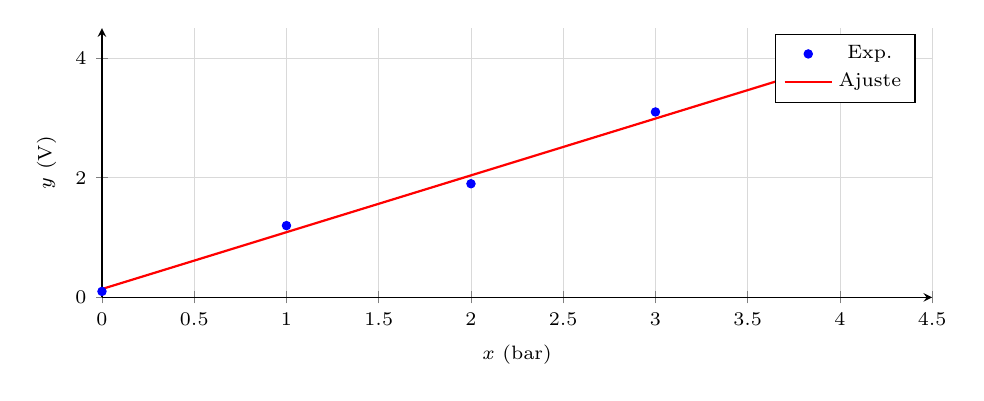
\begin{tikzpicture}
        \begin{axis}[
            width=\linewidth,
            height=5cm,
            xlabel={$x$ (bar)},
            ylabel={$y$ (V)},
            font=\scriptsize,
            grid=both,
            grid style={line width=.1pt, draw=gray!10},
            major grid style={line width=.2pt,draw=gray!30},
            axis lines=left,
            xmin=0, xmax=4.5,
            ymin=0, ymax=4.5
        ]
            % Puntos experimentales
            \addplot[
                only marks,
                mark=*,
                blue,
                mark size=1.5pt
            ] coordinates {
                (0, 0.1)
                (1, 1.2)
                (2, 1.9)
                (3, 3.1)
                (4, 3.9)
            };
            
            % Recta de ajuste: y = 0.95x + 0.14
            \addplot[
                thick,
                red,
                domain=0:4
            ] {0.95*x + 0.14};
            
            \legend{Exp., Ajuste}
        \end{axis}
    \end{tikzpicture}
    \caption[Representación de los puntos y la recta de ajuste calculada por el Método de los Mínimos Cuadrados.]{Representación de los puntos y la recta de ajuste calculada por el Método de los Mínimos Cuadrados.}\label{fig:grafico_ejemplo}
\end{marginfigure}

\subsection{Error de No Linealidad}\label{sec:error_no_linealidad}
Una vez calculados estos parámetros, el \emph{Error de No Linealidad}  se puede evaluar analizando el residuo máximo entre los valores medidos y los valores predichos por la recta de ajuste. El Error de No Linealidad se define como la máxima desviación de los puntos experimentales respecto a la recta de ajuste, expresado normalmente como porcentaje sobre el fondo de escala (\textit{Full Scale}, FS):

\begin{equation}
    \epsilon_{lin} = \frac{|y_i - (mx_i + b)|_{\max}}{y_{\max} - y_{\min}} \times 100\%
\end{equation}
para el ejemplo anterior, el error de no linealidad se calcularía evaluando el residuo máximo entre los valores medidos ($y_i$) y los valores predichos por la recta de ajuste ($mx_i + b$), y luego dividiendo por el rango total de salida ($y_{\max} - y_{\min}$) para obtener un porcentaje. Por lo tanto, el error de no linealidad se puede expresar como:

\begin{equation}
    \epsilon_{lin} = \frac{\max_i |y_i - (0.95x_i + 0.14)|}{3.9 - 0.1} \times 100\%
\end{equation}
donde $y_{\max} = 3.9$ V y $y_{\min} = 0.1$ V son los valores máximo y mínimo de la salida respectivamente. Este cálculo proporciona una medida cuantitativa de la desviación máxima de los puntos experimentales respecto a la recta de ajuste, lo que es crucial para evaluar la precisión del sensor en su rango de operación. Como $y_i$ valen 0.1, 1.2, 1.9, 3.1 y 3.9 V para $x_i$ igual a 0, 1, 2, 3 y 4 bar respectivamente, se evaluaría el residuo para cada punto y se identificaría el máximo para calcular el error de no linealidad. Así tenemos que el error de no linealidad se calcula evaluando el residuo para cada punto:
\begin{itemize}
    \item Para $x_0 = 0$ bar: $|0.1 - (0.95\cdot 0 + 0.14)| = |0.1 - 0.14| = 0.04$ V
    \item Para $x_1 = 1$ bar: $|1.2 - (0.95\cdot 1 + 0.14)| = |1.2 - 1.09| = 0.11$ V
    \item Para $x_2 = 2$ bar: $|1.9 - (0.95\cdot 2 + 0.14)| = |1.9 - 2.04| = 0.14$ V
    \item Para $x_3 = 3$ bar: $|3.1 - (0.95\cdot 3 + 0.14)| = |3.1 - 2.85| = 0.19$ V    
    \item Para $x_4 = 4$ bar: $|3.9 - (0.95\cdot 4 + 0.14)| = |3.9 - 3.64| = 0.21$ V
\end{itemize}
Por lo tanto, el residuo máximo es $0.21$ V para $x_4 = 4$ bar. Finalmente, el error de no linealidad se calcula como:
\begin{equation}
    \epsilon_{lin} = \frac{0.21}{3.9 - 0.1} \times 100\% \approx 5.38\%
\end{equation}
Esto indica que el error de no linealidad del sensor es aproximadamente del 5.38\% del fondo de escala, lo que proporciona una medida cuantitativa de la desviación máxima de los puntos experimentales respecto a la recta de ajuste, y es crucial para evaluar la precisión del sensor en su rango de operación. Un error de no linealidad del 5.38\% puede ser considerado aceptable o inaceptable dependiendo de los requisitos específicos de la aplicación para la cual se está utilizando el sensor. En aplicaciones donde se requiere alta precisión, este nivel de no linealidad podría ser problemático, mientras que en aplicaciones más tolerantes a la imprecisión, podría ser perfectamente adecuado. Por lo tanto, es importante evaluar este error en el contexto de la aplicación específica para determinar si el sensor cumple con los requisitos de precisión necesarios.




% \begin{itemize}
%     \item \emph{Error de No Linealidad}: Máxima desviación de los puntos experimentales respecto a la recta de ajuste, expresado normalmente como porcentaje sobre el fondo de escala (\textit{Full Scale}, FS).
%     \item \emph{Error de Histeresis}: Máxima diferencia en la salida para un mismo valor de entrada según el sentido de la variación (ascendente o descendente).
% \end{itemize}




\subsection{Recta de Referencia}
%que es la recta de referencia y como se define.

La recta de referencia, como se ilustra en la Figura~\ref{fig:recta_referencia}, es una linea que une el origen del sistema de coordenadas con el punto máximo de la salida. Esta recta se utiliza como una referencia para evaluar la linealidad y el comportamiento dinámico del sistema de medida. La elección de la recta de referencia es crucial, ya que puede influir en la interpretación de las características dinámicas del sensor, como la histéresis y la repetibilidad.

%ejemplo grafico de la recta de referencia y como se define.Dibujar una serie de puntos experimentales que no sean muy lineales y luego dibujar la recta de ajuste y la recta de referencia que los une. Explicar que esta recta se utiliza para evaluar la linealidad y el comportamiento dinámico del sistema de medida.
\begin{marginfigure}
    \centering
    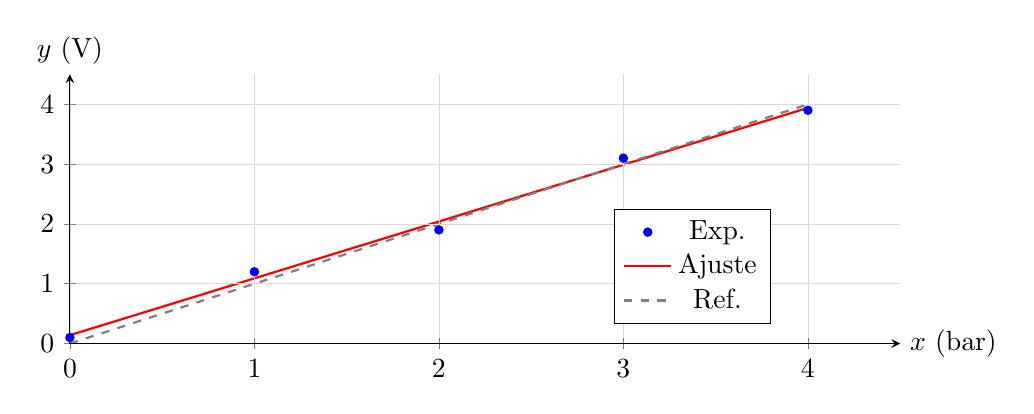
\begin{tikzpicture}
        \begin{axis}[
            width=\linewidth,
            height=5cm,
            xlabel={$x$ (bar)},
            ylabel={$y$ (V)},
            %font=\scriptsize,
            grid=both,
            grid style={line width=.1pt, draw=gray!10},
            major grid style={line width=.2pt,draw=gray!30},
            minor grid style={line width=.1pt,draw=gray!10},
            axis lines=left,
            every axis y label/.style={at=(current axis.above origin),anchor=south},
            every axis x label/.style={at=(current axis.right of origin),anchor=west},
            xmin=0, xmax=4.5,
            ymin=0, ymax=4.5,
            xtick={0,1,2,3,4},
            ytick={0,1,2,3,4},    
            xticklabels={$0$,$1$,$2$,$3$,$4$},
            yticklabels={$0$,$1$,$2$,$3$,$4$},
            enlargelimits=false, clip=false, axis on top,
            legend style={at={(0.75,0.5)}, anchor=north, legend columns=1},
        ]
            % Puntos experimentales
            \addplot[
                only marks,
                mark=*,
                blue,
                mark size=1.5pt
            ] coordinates {
                (0, 0.1)
                (1, 1.2)
                (2, 1.9)
                (3, 3.1)
                (4, 3.9)
            };
            
            % Recta de ajuste: y = 0.95x + 0.14
            \addplot[
                thick,
                red,
                domain=0:4
            ] {0.95*x + 0.14};
            
            % Recta de referencia: y = x
            \addplot[
                thick,
                dashed,
                gray,
                domain=0:4
            ] {x};
            \legend{Exp., Ajuste, Ref.}           
        \end{axis}       
    \end{tikzpicture}
    \caption[Recta de referencia y recta de ajuste]{
        Recta de referencia y recta de ajuste para una serie de puntos experimentales. 
    }\label{fig:recta_referencia}
\end{marginfigure}

% Como se define la recta de referencia. existen varias formas?
% la recta de referencia es una linea que une el origen del sistema de coordenadas con el punto máximo de la salida.

% Existen diferentes formas de definir la recta de referencia. La recta de referencia puede ser elegida basada en las siguientes características dinámicas:
% \begin{enumerate}
%     \item \emph{Linealidad de terminales}: Recta que une el origen y el punto máximo.
%     \item \emph{Linealidad a través de cero}: Obliga a que $b=0$.
%     \item \emph{Mejor recta de ajuste}: La obtenida por mínimos cuadrados (la más común).
% \end{enumerate}

\subsection{Histéresis y Repetibilidad}\label{sec:histeresis_repetibilidad}

Un sistema presenta \emph{histéresis} cuando la salida depende de la dirección en la que se alcanza la entrada (ascendente o descendente). Por ejemplo, si se aumenta la entrada $x$ desde un valor bajo hasta un valor alto, la salida $y$ puede seguir una curva diferente a la que se obtiene al disminuir $x$ desde el valor alto hasta el valor bajo. Esto se debe a que el sistema puede tener memoria o inercia, lo que provoca que la salida no solo dependa del valor actual de la entrada, sino también de su historia reciente. La histéresis es común en sensores magnéticos y mecánicos debido a la fricción o deformación elástica. En la Figura~\ref{fig:histeresis} se muestra un ejemplo gráfico del efecto de histéresis, donde la curva azul representa la variación ascendente de la entrada y la curva roja representa la variación descendente. La diferencia entre ambas curvas para el mismo rango de valores de entrada es una manifestación clara de la histéresis en el sistema.\marginnote{\textbf{Ejemplo de histéresis.} Un ejemplo típico de histéresis es el comportamiento de un motor de paso, donde la velocidad de rotación puede variar dependiendo de la dirección en la que se mueve el eje. Otro ejemplo típico de histéresis es el comportamiento de un termistor NTC\, donde la resistencia varía con la temperatura, pero la respuesta puede diferir dependiendo de si la temperatura está aumentando o disminuyendo, lo que es una manifestación de histéresis térmica.}

\begin{marginfigure}
    \centering
    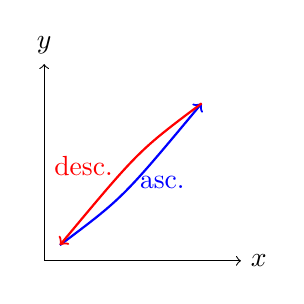
\begin{tikzpicture}
      \shorthandoff{>}
        \draw[->] (0,0) -- (2.5,0) node[right] {$x$};
        \draw[->] (0,0) -- (0,2.5) node[above] {$y$};
        % Curva ascendente
        \draw[blue, thick, ->] (0.2,0.2) .. controls (1,0.8) .. (2,2);
        % Curva descendente
        \draw[red, thick, ->] (2,2) .. controls (1.2,1.4) .. (0.2,0.2);
        \node[blue] at (1.5,1) {asc.};
        \node[red] at (.5,1.2) {desc.};
    \end{tikzpicture}
    \caption[Efecto de histéresis.]{Efecto de histéresis. Es común en sensores magnéticos y mecánicos debido a la fricción o deformación elástica.}\label{fig:histeresis}
\end{marginfigure}

%banda de Muerta

La \emph{banda muerta} es un fenómeno relacionado con la histéresis, donde existe un rango de valores de entrada que no produce ningún cambio en la salida. Esto es común en sistemas mecánicos con fricción o en sensores que requieren una fuerza mínima para activar la salida. Por ejemplo, en un reductor mecánico, puede haber una banda de muerta debido a la fricción interna, lo que significa que pequeñas variaciones en la entrada no se traducen en cambios en la salida hasta que se supera un umbral específico. En la Figura~\ref{fig:banda_muerta} se muestra un ejemplo gráfico de una banda de muerta, donde la curva azul representa la respuesta del sistema a variaciones de entrada. En el rango marcado como \emph{Banda de Muerta}, la salida permanece constante a pesar de las variaciones en la entrada, lo que ilustra claramente este fenómeno.\marginnote{\textbf{Ejemplo de Banda de Muerta.} Un ejemplo típico de banda de muerta es el comportamiento de un reductor mecánico, donde puede haber una banda de muerta debido a la fricción interna, lo que significa que pequeñas variaciones en la entrada no se traducen en cambios en la salida hasta que se supera un umbral específico. Otro ejemplo típico de banda de muerta es el comportamiento de un sensor de presión, donde puede haber una banda de muerta debido a la necesidad de superar una presión mínima para activar la salida del sensor.}

\begin{marginfigure}
    \centering
    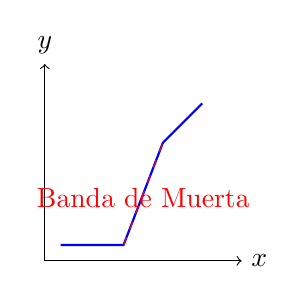
\begin{tikzpicture}
      \shorthandoff{>}
        \draw[->] (0,0) -- (2.5,0) node[right] {$x$};
        \draw[->] (0,0) -- (0,2.5) node[above] {$y$};
        % Curva con banda de muerta
        \draw[blue, thick] (0.2,0.2) -- (1,0.2) -- (1.5,1.5) -- (2,2);
        % Banda de muerta
        \draw[dashed, red] (1,0.2) -- (1.5,1.5);
        \node[red] at (1.25,0.8) {Banda de Muerta};
    \end{tikzpicture}
    \caption[Ejemplo de banda muerta.]{Ejemplo de banda muerta. Es común en sistemas mecánicos con fricción o en sensores que requieren una fuerza mínima para activar la salida.}\label{fig:banda_muerta}
\end{marginfigure}

La \emph{repetibilidad} es la capacidad de un sensor para entregar la misma salida al aplicar la misma entrada varias veces en periodos cortos de tiempo. Un sensor con buena repetibilidad producirá resultados consistentes bajo las mismas condiciones de prueba, lo que es crucial para aplicaciones donde se requiere alta precisión y confiabilidad. La repetibilidad se puede evaluar realizando múltiples mediciones con el mismo valor de entrada y analizando la variación en las salidas obtenidas. Un sensor con alta repetibilidad tendrá una desviación estándar baja en sus mediciones, lo que indica que las salidas son consistentes y confiables. En la Figura~\ref{fig:repetibilidad} se muestra un ejemplo gráfico de repetibilidad, donde se realizan varias mediciones con el mismo valor de entrada. La dispersión de los puntos alrededor de la media indica el nivel de repetibilidad del sensor, siendo una dispersión menor indicativa de una mejor repetibilidad.\marginnote{\textbf{Ejemplo de repetibilidad.} Un ejemplo típico de repetibilidad es el comportamiento de un sensor de temperatura, donde se espera que el sensor entregue la misma salida para la misma temperatura en múltiples mediciones realizadas en periodos cortos de tiempo. Otro ejemplo típico de repetibilidad es el comportamiento de un sensor de presión, donde se espera que el sensor entregue la misma salida para la misma presión en múltiples mediciones realizadas en periodos cortos de tiempo.} 

% \begin{margintable}
%     \centering
%     %\footnotesize
%     \begin{tabular}{c c}
%         \toprule
%         Medición (20 ºC) & Salida (V) \\
%         \midrule
%         1 & 2.0 \\
%         2 & 1.9 \\
%         3 & 2.1 \\
%         4 & 2.0 \\
%         5 & 1.95 \\
%         \bottomrule
%         \\
%     \end{tabular}
%     \caption{Ejemplo de repetibilidad. Se muestran varias mediciones con el mismo valor de entrada y la variación en las salidas obtenidas para evaluar la repetibilidad del sensor.}
%     \label{tab:repetibilidad}
% \end{margintable}

\begin{marginfigure}
    \centering
    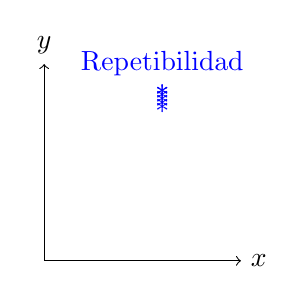
\begin{tikzpicture}
      \shorthandoff{>}
        \draw[->] (0,0) -- (2.5,0) node[right] {$x$};
        \draw[->] (0,0) -- (0,2.5) node[above] {$y$};
        % Puntos de repetibilidad dibujados con node como puntos azules 
        \node[blue] at (1.5,2.1) {*};
        \node[blue] at (1.5,2.0) {*};
        \node[blue] at (1.5,1.9) {*};
        \node[blue] at (1.5,2.1) {*};
        \node[blue] at (1.5,2.05) {*};
        \node[blue] at (1.5,1.95) {*};        
        \node[blue] at (1.5,2.5) {Repetibilidad};
    \end{tikzpicture}
    \caption[Ejemplo de repetibilidad.]{Ejemplo de repetibilidad. Un sensor con buena repetibilidad producirá resultados consistentes bajo las mismas condiciones de prueba.}\label{fig:repetibilidad}
\end{marginfigure}

\subsection{Error de Histéresis}


Además, el \emph{Error de Histeresis} se puede evaluar comparando las salidas para un mismo valor de entrada según el sentido de la variación (ascendente o descendente). Este error se define como la máxima diferencia en la salida para un mismo valor de entrada según el sentido de la variación, y se expresa también como porcentaje sobre el fondo de escala:

\begin{equation}    
    \epsilon_{his} = \frac{|y_{asc} - y_{desc}|_{\max}}{y_{\max} - y_{\min}} \times 100\%
\end{equation}
donde $y_{asc}$ y $y_{desc}$ son las salidas correspondientes a un mismo valor de entrada durante la variación ascendente y descendente respectivamente. Este cálculo proporciona una medida cuantitativa de la diferencia máxima en la salida para un mismo valor de entrada según el sentido de la variación, lo que es fundamental para evaluar la estabilidad y confiabilidad del sensor en aplicaciones donde se esperan cambios frecuentes en la magnitud medida.

\subsection{Rango de Entrada y Saturación}

Todo sistema de medida está diseñado para operar dentro de un intervalo específico de la magnitud de entrada $[x_{\min}, x_{\max}]$. El Fondo de Escala (Full Scale, FS) es la diferencia entre el valor máximo y el valor mínimo medible: $FS = x_{\max} - x_{\min}$. Define la capacidad total del instrumento.
    
La saturación es una característica no lineal que ocurre cuando la entrada excede los límites de diseño. En este estado, la salida $y$ deja de responder a incrementos de la entrada $x$, permaneciendo constante en un valor máximo ($y_{sat}$). En la Figura~\ref{fig:saturacion} se muestra un ejemplo gráfico de saturación, donde la curva azul representa la relación entre la entrada $x$ y la salida $y$. En la zona lineal (hasta $x_{sat}$), la salida aumenta proporcionalmente a la entrada. Sin embargo, una vez que se alcanza el punto de saturación ($x_{sat}$), la salida se mantiene constante en $y_{sat}$, independientemente de cualquier aumento adicional en la entrada. Esto ilustra claramente cómo la saturación limita el rango operativo del sistema de medida y afecta su capacidad para seguir cambios en la magnitud física más allá de ciertos límites.\marginnote{\textbf{Saturación:} Un sistema debe diseñarse para que su rango dinámico de trabajo nunca alcance la saturación, ya que en esa zona la sensibilidad es nula ($S = dy/dx = 0$) y la información de la magnitud física se pierde por completo.
}

\begin{marginfigure}
    \centering
    \shorthandoff{>}
    \begin{tikzpicture}
        \begin{axis}[
            width=\linewidth, height=4.5cm,
            xlabel={$x$}, ylabel={$y$},
            font=\scriptsize,
            axis lines=left,
            xmin=0, xmax=5, ymin=0, ymax=3.5,
            xtick={3}, xticklabels={$x_{sat}$},
            ytick={3}, yticklabels={$y_{sat}$},
            every axis y label/.style={at=(current axis.above origin),anchor=south},
            every axis x label/.style={at=(current axis.right of origin),anchor=west},
        ]
            % Zona lineal
            \addplot[thick, blue, domain=0:3] {x};
            % Zona de saturación
            \addplot[thick, red, domain=3:5] {3};
            % Línea discontinua ideal (prolongación)
            \addplot[dashed, gray, domain=3:4.5] {x};
            
            \node[blue, rotate=43] at (axis cs:1.2,1.6) {Zona Lineal};
            \node[red] at (axis cs:4,3.2) {Saturación};
        \end{axis}
    \end{tikzpicture}
    \caption[Característica de saturación.]{Característica de saturación. Físicamente, suele estar impuesta por los límites de alimentación de la electrónica o la deformación máxima del material del sensor.}\label{fig:saturacion}
\end{marginfigure}

\subsection{Efecto de Carga e Impedancias}\label{sub:efecto_carga_general}

Al conectar la salida de una etapa con la entrada de la siguiente --el sensor con el acondicionador, el acondicionador con el convertidor, el instrumento con el sistema de registro-- no se unen dos terminales ideales, sino una fuente con impedancia de salida $R_{out}$ y una carga con impedancia de entrada $R_{in}$. Ambas forman un divisor de tensión, y la señal que llega al receptor ya no es la que salió de la fuente:
\begin{equation}\label{eq:error_carga}
    v_{rx} = v_{tx}\,\frac{R_{in}}{R_{in} + R_{out}}, \qquad \frac{\Delta v}{v_{tx}} \approx -\frac{R_{out}}{R_{in}} \quad \text{si } R_{in} \gg R_{out}
\end{equation}
La regla de diseño es, por tanto, que la impedancia de entrada sea mucho mayor que la de salida: dos órdenes de magnitud de diferencia dejan un error del orden del \SI{1}{\percent}. La gravedad del efecto depende de la impedancia de la fuente, y por eso conviene conocerla antes de elegir la etapa siguiente: un sensor pasivo de \SI{1}{\kilo\ohm} no puede leerse con una entrada de \SI{1}{\kilo\ohm} --se pierde la mitad de la señal--, mientras que un termopar de unos pocos ohmios apenas acusa una entrada de \SI{10}{\kilo\ohm}. En los sensores resistivos este mismo efecto es el que obliga a las configuraciones de tres y cuatro hilos (Figura~\ref{fig:efecto_carga}) y en el acondicionamiento es la razón de ser de la etapa de entrada del amplificador de instrumentación (Sección~\ref{sec:inamp}).

\marginnote{\textbf{Efecto de carga en cifras:} una fuente de \SI{1}{\kilo\ohm} leída por una entrada de \SI{100}{\kilo\ohm} pierde el \SI{1}{\percent} de la señal; con una entrada de \SI{1}{\mega\ohm}, pierde el \SI{0.1}{\percent}. Como el error es sistemático y depende de una impedancia que a su vez cambia con la temperatura, no se corrige en el software: se combate con una etapa de entrada de alta impedancia, como un seguidor de tensión o un amplificador de instrumentación.}

\section{Características Dinámicas}\label{sec:caract_dinamicas} 

Las características dinámicas describen el comportamiento de un sistema de medida cuando la magnitud física varía con el tiempo. A diferencia de las características estáticas, que se centran en la relación entre entrada y salida en condiciones de equilibrio o variaciones lentas, las características dinámicas analizan cómo el sistema responde a cambios rápidos en la magnitud medida, incluyendo aspectos como la velocidad de respuesta, la estabilidad y la capacidad para seguir señales de alta frecuencia.

Las características dinámicas analizan la respuesta del sistema cuando la entrada $x(t)$ varía rápidamente. Matemáticamente, se modelan mediante una ecuación diferencial lineal de coeficientes constantes:

\begin{equation}
    a_n \frac{d^n y}{dt^n} + \cdots + a_1 \frac{dy}{dt} + a_0 y = b_m \frac{d^m x}{dt^m} + \cdots + b_0 x
\end{equation}

\subsection{Sistema de Orden 0}
Un sistema de orden 0 es un sensor ideal. La salida sigue a la entrada instantáneamente sin retardo ni error dinámico como se muestra en la Figura~\ref{fig:orden_0}. Su ecuación es:
\[ y(t) = K \cdot x(t) \]
donde $K$ es una constante de ganancia. La sensibilidad estática $K     = b_0/a_0$ es la sensibilidad estática.
%Figura de larespuesta escalon de un sistema de orden 0, que es una linea recta que sigue a la entrada sin retardo ni error dinamico.
\begin{marginfigure}
    \centering
    \begin{tikzpicture}
        \begin{axis}[ 
            width=\linewidth, height=4.5cm,
            xlabel={$t$}, ylabel={$y(t)$},
            font=\scriptsize,
            axis lines=left,
            ymin=0, ymax=1.5,
            every axis y label/.style={at=(current axis.above origin),anchor=south},
            every axis x label/.style={at=(current axis.right of origin),anchor=west},
            %xtick={1}, %xticklabels={$\tau$},
            ytick={1,1.01}, yticklabels={K}
        ]
           % ENTRADA (Escalón en t=0)
            \addplot[thick, red, dashed, domain=0:4] {1.01};
            %\addlegendentry{Entrada $x(t)$}

            % SALIDA (Orden 0: Sigue instantáneamente)
            % Usamos una línea sólida azul justo encima
            \addplot[thick, blue, domain=0:4] {1};
            %\addlegendentry{Salida $y(t)$}
        \end{axis}
    \end{tikzpicture}
    \caption[Respuesta al escalón de un sistema de orden 0.]{Respuesta al escalón de un sistema de orden 0. La salida sigue a la entrada instantáneamente sin retardo ni error dinámico.}\label{fig:orden_0}
\end{marginfigure}

\subsection{Sistema de Primer Orden}
Corresponde a sensores con almacenamiento de energía (ej.\ una capacidad térmica de un termómetro o condensador en un circuito). En este caso la salida $y(t)$ depende de la entrada $x(t)$ y de la constante de tiempo $\tau$. Matemáticamente, se modela mediante una ecuación diferencial lineal de primer orden. Su ecuación es:
\[ \tau \frac{dy(t)}{dt} + y(t) = K \cdot x(t) \]
donde $K$ es una constante de ganancia. La sensibilidad estática $K = b_0/a_0$ es la sensibilidad estática. En la Figura~\ref{fig:primer_orden} se muestra la respuesta al escalón de un sistema de primer orden. La respuesta al escalón de un sistema de primer orden es una curva exponencial que se aproxima a un valor final $K \cdot x(t)$ con una constante de tiempo $\tau$ que es un parámetro crucial que define la rapidez del sensor, ya que determina cuánto tiempo tarda la salida en responder a un cambio en la entrada. Un valor de $\tau$ más pequeño indica una respuesta más rápida, mientras que un valor de $\tau$ más grande indica una respuesta más lenta.\marginnote{\textbf{Constante de Tiempo ($\tau$):} Es el parámetro que define la rapidez del sensor. Representa el tiempo necesario para que la salida alcance el \qty{63.2}{\percent} de su valor final ante un escalón.
}

% Figura que muestra el escalon en rojo y en azul la respuesta al escalon de un sistema de primer orden, que es una curva exponencial que se aproxima a un valor final $K \cdot x(t)$ con una constante de tiempo $\tau$ que determina la rapidez de la respuesta. Las líneas punteadas indican el tiempo $\tau$ necesario para que la salida alcance el \SI{63.2}{\percent} de su valor final. La constante de tiempo $\tau$ es un parámetro crucial que define la rapidez del sensor, ya que determina cuánto tiempo tarda la salida en responder a un cambio en la entrada. Un valor de $\tau$ más pequeño indica una respuesta más rápida, mientras que un valor de $\tau$ más grande indica una respuesta más lenta.
\begin{marginfigure}
    \centering
    \begin{tikzpicture}
        \begin{axis}[
            width=\linewidth, height=4.5cm,
            xlabel={$t$}, ylabel={$y(t)$},
            %font=\scriptsize,
            %rango del eje y es 0 a 2
            ymin=0, ymax=1.5,
            axis lines=left,
            every axis y label/.style={at=(current axis.above origin),anchor=south},
            every axis x label/.style={at=(current axis.right of origin),anchor=west},
            xtick={1}, xticklabels={$\tau$},
            ytick={0.63, 1}, yticklabels={0.63K, K}
        ]
            % Dibujar la curva azul expomnencial de la respuesta al escalón
            \addplot[thick, blue, domain=0:4, samples=50] {1-exp(-x)};
            % Dibujar líneas punteadas para indicar el tiempo $\tau$ y el valor 0.63K
            % Líneas punteadas de la constante de tiempo
            \draw[dashed, gray] (axis cs:1,0) -- (axis cs:1,0.632);
            \draw[dashed, gray] (axis cs:0,0.632) -- (axis cs:1,0.632);
            \addplot[thick, red, dashed, domain=0:4] {1};
        \end{axis}
    \end{tikzpicture}
    \caption[Respuesta al escalón de un sistema de 1er orden.]{Respuesta al escalón de un sistema de 1er orden. La curva azul representa la salida $y(t)$ que se aproxima a su valor final $K \cdot x(t)$ de manera exponencial, y las líneas punteadas indican el tiempo $\tau$ necesario para que la salida alcance el \SI{63.2}{\percent} de su valor final. }\label{fig:primer_orden}
\end{marginfigure}

\subsection{Sistema de Segundo Orden}\label{sec:segundo_orden}
Corresponde a sensores con almacenamiento de energía y  con oscilaciones (ej.\ un sistema mecánico con masa, resorte y amortiguador, como el que se ilustra en la Figura~\ref{fig:masa_resorte}). Este sistema mecánico se rige por la segunda ley de Newton, resultando en la ecuación diferencial de segundo orden. 
\begin{equation}\label{eq:segundo_orden}
m \frac{d^2y(t)}{dt^2} + c \frac{dy(t)}{dt} + ky(t) = F(t)
\end{equation}
donde $m$ es la masa, $c$ es el coeficiente de amortiguamiento, $k$ es la constante del resorte y $F(t)$ es la fuerza externa aplicada. En esta ecuación, el término $m \frac{d^2y(t)}{dt^2}$ representa la inercia del sistema, el término $c \frac{dy(t)}{dt}$ representa la fuerza de amortiguamiento que se opone al movimiento, y el término $ky(t)$ representa la fuerza restauradora del resorte. La respuesta dinámica de este sistema puede presentar oscilaciones dependiendo de los valores de $m$, $c$ y $k$, lo que hace que su análisis sea más complejo en comparación con los sistemas de orden 0 y 1.
%
% Mostrar figura de un sistema mecánico con masa, resorte y amortiguador.
\begin{marginfigure}
    \centering
    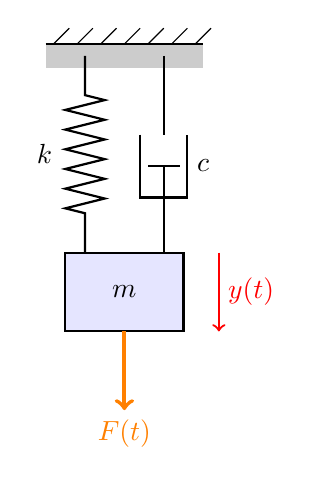
\begin{tikzpicture}[every node/.style={draw,outer sep=0pt,thick}]
        \shorthandoff{>}
        % Soporte superior (Techo)
        \node (ceiling) [shape=rectangle,fill=black!20,minimum width=2cm,minimum height=0.3cm,draw=none] at (0,0) {};
        \draw[thick] (-1,0.15) -- (1,0.15);
        \foreach \x in {-0.9,-0.6,...,0.9}
            \draw (\x,0.15) -- (\x+0.2,0.35);

        % Masa
        \node (M) [shape=rectangle,fill=blue!10,minimum width=1.5cm,minimum height=1cm] at (0,-3) {$m$};

        % Resorte (Spring) - Usando decoración zigzag
        \draw[decoration={zigzag,amplitude=2.5mm,segment length=2.5mm,post length=5mm,pre length=5mm},decorate,thick] 
            (-0.5,0) -- (-0.5,-2.5) node[midway,left=3mm,draw=none] {$k$};

        % Amortiguador (Damper) - Dibujo manual del pistón
        \begin{scope}[xshift=0.5cm]
            % Parte fija (cilindro)
            \draw[thick] (0,0) -- (0,-1);
            \draw[thick] (-0.3,-1) -- (-0.3,-1.8) -- (0.3,-1.8) -- (0.3,-1);
            % Parte móvil (pistón)
            \draw[thick] (0,-2.5) -- (0,-1.4);
            \draw[thick] (-0.2,-1.4) -- (0.2,-1.4);
            \node[draw=none] at (0.5,-1.4) {$c$};
        \end{scope}

        % Coordenada de desplazamiento
        \draw[->,thick,red] (1.2,-2.5) -- (1.2,-3.5) node[midway,right,draw=none] {$y(t)$};
        
        % Fuerza externa (opcional)
        \draw[->,line width=1.5pt,orange] (0,-3.5) -- (0,-4.5) node[below,draw=none] {$F(t)$};

    \end{tikzpicture}
    \caption[Sistema mecánico de segundo orden.]{Sistema mecánico de segundo orden. Los parámetros $m$ (masa), $k$ (constante elástica) y $c$ (coeficiente de amortiguamiento) definen la respuesta dinámica del sensor.}\label{fig:masa_resorte}
\end{marginfigure}
%
Comparando la expresión~\eqref{eq:segundo_orden} con la forma normalizada de un sistema de segundo orden:
\begin{equation}    
\frac{d^2 y(t)}{dt^2} + 2\zeta \omega_n \frac{dy(t)}{dt} + \omega_n^2 y(t) = \frac{F(t)}{m}
\end{equation}
podemos obtener las relaciones fundamentales para el diseño de sensores de segundo orden:
\begin{equation}
\omega_n = \sqrt{\frac{k}{m}} \quad  \quad \zeta = \frac{c}{2\sqrt{km}} \quad \quad K = \frac{1}{m\omega_n^2} = \frac{1}{k}
\end{equation}
donde $\omega_n$ es la \emph{frecuencia natural} del sistema, $\zeta$ es el \emph{factor de amortiguamiento} y $K$ es la sensibilidad estática.  

La frecuencia natural $\omega_n$ influye en la rapidez de la respuesta, siendo una frecuencia más alta indicativa de una respuesta más rápida. Esta respuesta al escalón de un sistema de segundo orden puede presentar oscilaciones dependiendo del valor del factor de amortiguamiento $\zeta$.%\marginnote{\textbf{Factor de Amortiguamiento ($\zeta$):} Es un parámetro que determina el tipo de respuesta del sistema. Si $\zeta < 1$, el sistema es subamortiguado y presenta oscilaciones. Si $\zeta = 1$, el sistema es críticamente amortiguado y alcanza su valor final sin oscilar. Si $\zeta > 1$, el sistema es sobreamortiguado y se aproxima a su valor final de manera exponencial sin oscilar.}
\begin{enumerate}
    \item Si $\zeta < 1$, el sistema es subamortiguado y la salida oscila antes de estabilizarse en su valor final.
    \item Si $\zeta = 1$, el sistema es críticamente amortiguado y la salida alcanza su valor final sin oscilar.
    \item Si $\zeta > 1$, el sistema es sobreamortiguado y la salida se aproxima a su valor final de manera exponencial.
\end{enumerate}
%\marginnote{\textbf{Frecuencia Natural ($\omega_n$):} Es un parámetro que influye en la rapidez de la respuesta del sistema. Una frecuencia natural más alta indica una respuesta más rápida, mientras que una frecuencia natural más baja indica una respuesta más lenta.}

 %

%
En la Figura~\ref{fig:segundo_orden} se muestra la respuesta al escalón de un sistema de segundo orden. En el caso de un sistema de segundo orden \emph{subamortiguado}, la ecuación que gobierna la respuesta al escalón es:
\begin{equation}
    y(t) = K \left( 1 - e^{-\zeta \omega_n t} \left( \cos(\omega_d t) + \frac{\zeta}{\sqrt{1-\zeta^2}} \sin(\omega_d t) \right) \right)
\end{equation}
donde $\omega_d = \omega_n \sqrt{1-\zeta^2}$ es la frecuencia de oscilación amortiguada. En esta ecuación, el término $e^{-\zeta \omega_n t}$ representa la envolvente de decaimiento de las oscilaciones, mientras que la combinación de las funciones trigonométricas describe la naturaleza oscilatoria del sistema. La sobreoscilación máxima $M_p$ se puede calcular como:
\begin{equation}
    M_p = e^{-\frac{\pi \zeta}{\sqrt{1-\zeta^2}}}
\end{equation}
que representa la máxima desviación de la salida respecto al valor final durante las oscilaciones. La frecuencia de oscilación amortiguada $\omega_d$ también influye en la rapidez de las oscilaciones, siendo una frecuencia más alta indicativa de oscilaciones más rápidas. En resumen, la respuesta al escalón de un sistema de segundo orden subamortiguado se caracteriza por una combinación de un crecimiento exponencial amortiguado y oscilaciones sinusoidales, donde la magnitud de la sobreoscilación y la frecuencia de las oscilaciones dependen del factor de amortiguamiento $\zeta$ y la frecuencia natural $\omega_n$ del sistema.
% Figura que muestra el escalon en rojo y en azul la respuesta al escalon de un sistema de segundo orden, que puede presentar oscilaciones dependiendo del valor del factor de amortiguamiento $\zeta$. Si $\zeta < 1$, el sistema es subamortiguado y la salida oscila antes de estabilizarse en su valor final. Si $\zeta = 1$, el sistema es críticamente amortiguado y la salida alcanza su valor final sin oscilar. Si $\zeta > 1$, el sistema es sobreamortiguado y la salida se aproxima a su valor final de manera exponencial sin oscilar. La frecuencia natural $\omega_n$ también influye en la rapidez de la respuesta, siendo una frecuencia más alta indicativa de una respuesta más rápida.
\begin{marginfigure}
    \centering
    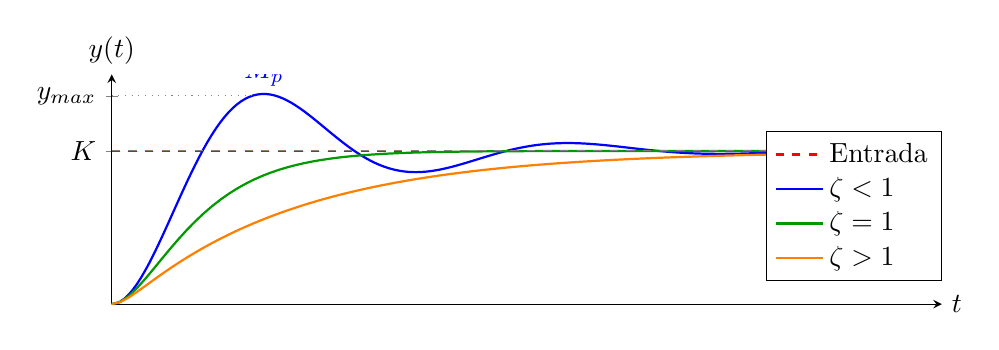
\begin{tikzpicture}
        \begin{axis}[
            width=\linewidth, height=4.5cm,
            xlabel={$t$}, ylabel={$y(t)$},
            %font=\scriptsize,
            ymin=0, ymax=1.5, xmin=0, xmax=6,
            axis lines=left,
            % IMPORTANTE: Usar radianes para las funciones trigonométricas
            trig format plots=rad, 
            every axis y label/.style={at=(current axis.above origin),anchor=south},
            every axis x label/.style={at=(current axis.right of origin),anchor=west},
            % Etiquetas correctas para 2º orden
            xtick=\empty,
            ytick={1, 1.36}, yticklabels={$K$, $y_{max}$},
            legend style={at={(1,0.1)}, anchor=south east, cells={anchor=west}}
        ]
            % 1. ESCALÓN DE ENTRADA
            \addplot[thick, red, dashed, domain=0:6] {1};
            \addlegendentry{Entrada}

            % 2. SUBAMORTIGUADO (zeta = 0.3, wn = 3) - CORRECTO
            \addplot[thick, blue, domain=0:6, samples=200] 
                {1 - exp(-0.9*x) * (cos(2.86*x) + 0.314*sin(2.86*x))};
            \addlegendentry{$\zeta < 1$}
            
            % Marcador de Sobreoscilación para el azul
            \draw[dotted, gray] (axis cs:0,1.36) -- (axis cs:1.1,1.36);
            \node[anchor=south, blue] at (axis cs:1.1, 1.36) {$M_p$};

            % 3. CRÍTICAMENTE AMORTIGUADO (zeta = 1, wn = 3)
            % Fórmula: y(t) = 1 - (1 + wn*t)*exp(-wn*t)
            \addplot[thick, green!60!black, domain=0:6, samples=100] 
                {1 - (1 + 3*x)*exp(-3*x)};
            \addlegendentry{$\zeta = 1$}
            
            % 4. SOBREAMORTIGUADO (zeta = 2, wn = 3)
            % Fórmula: suma de dos exponenciales reales
            \addplot[thick, orange, domain=0:6, samples=100] 
                {1 - 1.077*exp(-0.804*x) + 0.077*exp(-11.19*x)};
            \addlegendentry{$\zeta > 1$}

            % Línea de valor final
            \draw[dashed, gray] (axis cs:0,1) -- (axis cs:6,1);
        \end{axis}
    \end{tikzpicture}
    \caption[Respuesta al escalón de un sistema de segundo orden.]{Respuesta al escalón de un sistema de segundo orden. Las curvas representan las salidas $y(t)$ que puedes presentar oscilaciones dependiendo del valor del factor de amortiguamiento $\zeta$. En este caso, se muestra un sistema subamortiguado ($\zeta < 1$) donde la salida oscila antes de estabilizarse en su valor final; un sistema críticamente amortiguado ($\zeta = 1$) donde la salida alcanza su valor final sin oscilar; y un sistema sobreamortiguado ($\zeta > 1$) donde la salida se aproxima a su valor final de manera exponencial sin oscilar.}\label{fig:segundo_orden}
\end{marginfigure}


En el caso de un sistema de segundo orden \emph{críticamente amortiguado}, la ecuación que gobierna la respuesta al escalón es:
\begin{equation}
    y(t) = K \left( 1 - (1 + \omega_n t) e^{-\omega_n t} \right)
\end{equation}
donde $\omega_n$ es la frecuencia natural del sistema. En esta ecuación, el término $(1 + \omega_n t) e^{-\omega_n t}$ representa la combinación de un crecimiento lineal y un decaimiento exponencial que caracteriza la respuesta de un sistema críticamente amortiguado. La salida $y(t)$ se aproxima a su valor final $K$ sin presentar oscilaciones, y la rapidez con la que alcanza el valor final está determinada por la frecuencia natural $\omega_n$. En resumen, la respuesta al escalón de un sistema de segundo orden críticamente amortiguado se caracteriza por una aproximación suave al valor final sin oscilaciones, donde la rapidez de la respuesta está influenciada por la frecuencia natural del sistema.    

Y por último, en el caso de un sistema de segundo orden \emph{sobreamortiguado}, las raíces de la ecuación característica son reales y distintas. La respuesta al escalón no presenta oscilaciones y es más lenta que en el caso crítico, la ecuación que gobierna la respuesta al escalón es:
\begin{equation}
y(t) = K \left( 1 - \frac{s_2}{s_2 - s_1} e^{s_1 t} + \frac{s_1}{s_2 - s_1} e^{s_2 t} \right)
\end{equation}
donde $s_1$ y $s_2$ son las raíces reales de la ecuación característica dada por:
\begin{equation}
s_{1,2} = -\zeta \omega_n \pm \omega_n \sqrt{\zeta^2 - 1}
\end{equation}
En esta ecuación, el término $\frac{s_2}{s_2 - s_1} e^{s_1 t}$ y $\frac{s_1}{s_2 - s_1} e^{s_2 t}$ representan la combinación de dos exponenciales reales que caracterizan la respuesta de un sistema sobreamortiguado. La salida $y(t)$ se aproxima a su valor final $K$ de manera más lenta que en el caso críticamente amortiguado, y no presenta oscilaciones. La rapidez con la que alcanza el valor final está determinada por las raíces $s_1$ y $s_2$, que a su vez dependen del factor de amortiguamiento $\zeta$ y la frecuencia natural $\omega_n$ del sistema.\marginnote{\textbf{Raíces Reales:} En un sistema de segundo orden sobreamortiguado, las raíces de la ecuación característica son reales y negativas, lo que garantiza que los términos exponenciales decaigan hacia cero, permitiendo que la salida alcance el valor final $K$ de manera lenta que en el caso críticamente amortiguado. Las raíces reales son determinadas por el factor de amortiguamiento $\zeta$ y la frecuencia natural $\omega_n$ del sistema.}

\subsection{Ejemplo de Cálculo de la Respuesta al Escalón de un Sistema de Segundo Orden con $\zeta = 0.3$ y $\omega_n = 3$}\label{sec:ejemplo_segundo_orden}

A modo de ejemplo, en la Figura~\ref{fig:ejemplo_segundo_orden} se muestra el cálculo de la respuesta al escalón de un sistema de segundo orden con $\zeta = 0.3$ y $\omega_n = 3$. El sistema es subamortiguado ($\zeta < 1$) y la salida oscila antes de estabilizarse en su valor final. La curva azul representa la salida $y(t)$ que se aproxima a su valor final $K$ de manera exponencial amortiguada y oscilatoria, donde la magnitud de la sobreoscilación $M_p$ y la frecuencia de las oscilaciones dependen del factor de amortiguamiento $\zeta=0.3$ y la frecuencia natural $\omega_n=3$ del sistema. En este caso, se observa que la salida oscila antes de estabilizarse en su valor final, lo que es característico de un sistema subamortiguado. 

La magnitud de la sobreoscilación $M_p$ se calcula de la siguiente forma:
\begin{equation}
    M_p = e^{-\frac{\pi \zeta}{\sqrt{1-\zeta^2}}} = e^{-\frac{\pi \cdot 0.3}{\sqrt{1-0.3^2}}} \approx 0.372
\end{equation}
lo que indica que la salida alcanza un máximo de aproximadamente $1.37K$ antes de estabilizarse en su valor final $K$. La frecuencia de las oscilaciones amortiguadas $\omega_d$ se calcula como:
\begin{equation}
    \omega_d = \omega_n \sqrt{1-\zeta^2} = 3 \sqrt{1-0.3^2} \approx \SI{2.86}{rad/s}
\end{equation}
A partir de este valor, podemos predecir el instante en el que ocurrirá el primer pico (tiempo de pico, $t_p$):
\begin{equation}
    t_p = \frac{\pi}{\omega_d} = \frac{\pi}{2.86} \approx \SI{1.1}{s}
\end{equation}
La caracterización dinámica obtenida para el sistema ($\zeta = 0.3$ y $\omega_n = \SI{3}{rad/s}$) permite extraer conclusiones críticas sobre la calidad de la medida en régimen transitorio:

\begin{itemize}
    \item \emph{Frecuencia Amortiguada ($\omega_d$)}: El valor de $\omega_d \approx \SI{2.86}{rad/s}$ determina la \textit{periodicidad del transitorio}. Físicamente, representa la velocidad a la que el sistema oscila antes de alcanzar el equilibrio. Una $\omega_d$ más elevada es un indicador directo de una \emph{respuesta más rápida}, reduciendo el tiempo necesario para que el sensor reaccione inicialmente, aunque puede comprometer la estabilidad si el amortiguamiento es bajo.
    
    \item \emph{Sobreoscilación Máxima ($M_p$)}: El resultado de \SI{37.2}{\percent} indica que el sensor experimentará un \textit{error dinámico temporal} considerable, superando el valor real de la magnitud física en más de un tercio de su valor de estado estacionario ($K$). 
    
    \item \emph{Tiempo de Pico ($t_p$)}: Este error máximo ocurre exactamente a los \SI{1.1}{s} tras la aparición del escalón. Para un ingeniero de instrumentación, este dato es vital: cualquier captura de datos (muestreo) realizada cerca de este instante daría una lectura errónea y sobredimensionada de la magnitud real.
\end{itemize}
\marginnote{\textbf{Compromiso de Diseño:} En instrumentación, existe un \textit{trade-off} constante. Aumentar la rapidez (subir $\omega_n$) suele desplazar el tiempo de pico $t_p$ hacia la izquierda (más rápido), pero si no se controla el factor de amortiguamiento $\zeta$, la sobreoscilación $M_p$ puede dañar el sistema o saturar las etapas de amplificación posteriores.}

En resumen, el sistema analizado es capaz de seguir cambios con una rapidez moderada ($\omega_d \approx \SI{2.86}{rad/s}$), pero a costa de un transitorio oscilatorio pronunciado que requiere esperar al menos hasta el \emph{tiempo de establecimiento} ($t_s$) para que la medida se considere válida y dentro de una banda de error aceptable.

%ejemplo de calculo de la respuesta al escalon de un sistema de segundo orden subamortiguado, con $\zeta = 0.3$ y $\omega_n = 3$.
\begin{marginfigure}
    \centering
    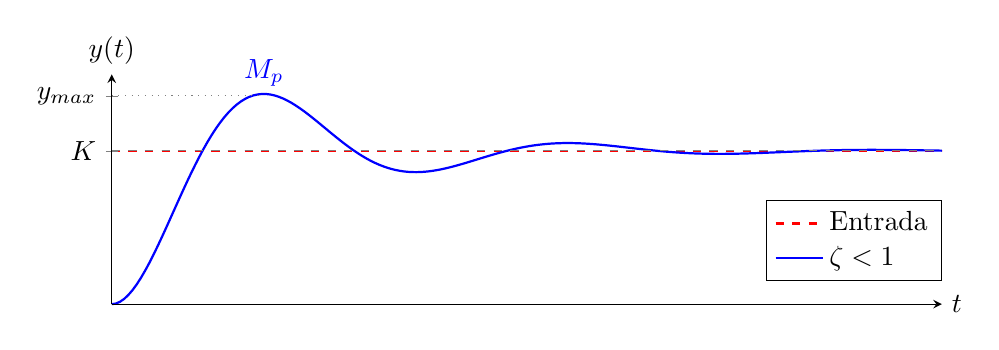
\begin{tikzpicture}
        \begin{axis}[
            width=\linewidth, height=4.5cm,
            xlabel={$t$}, ylabel={$y(t)$},
            %font=\scriptsize,
            ymin=0, ymax=1.5, xmin=0, xmax=6,            
            axis lines=left,            
            % IMPORTANTE: Usar radianes para las funciones trigonométricas
            trig format plots=rad,            
            every axis y label/.style={at=(current axis.above origin),anchor=south},            
            every axis x label/.style={at=(current axis.right of origin),anchor=west},            
            enlargelimits=false, clip=false, axis on top,
            legend style={at={(1,0.1)}, anchor=south east, cells={anchor=west}},
            % Etiquetas correctas para 2º orden
            xtick=\empty,
            ytick={1, 1.36}, yticklabels={$K$, $y_{max}$},
        ]
            % 1. ESCALÓN DE ENTRADA
            \addplot[thick, red, dashed, domain=0:6] {1};
            \addlegendentry{Entrada}

            % 2. SUBAMORTIGUADO (zeta = 0.3, wn = 3) - CORRECTO
            \addplot[thick, blue, domain=0:6, samples=200] 
                {1 - exp(-0.9*x) * (cos(2.86*x) + 0.314*sin(2.86*x))};
            \addlegendentry{$\zeta < 1$}
            
            % Marcador de Sobreoscilación para el azul
            \draw[dotted, gray] (axis cs:0,1.36) -- (axis cs:1.1,1.36);
            \node[anchor=south, blue] at (axis cs:1.1, 1.36) {$M_p$};

            % Línea de valor final
            \draw[dashed, gray] (axis cs:0,1) -- (axis cs:6,1);
        \end{axis}
    \end{tikzpicture}
    \caption[Respuesta al escalón de un sistema de segundo orden.]{Ejemplo de cálculo de la respuesta al escalón de un sistema de segundo orden subamortiguado, con $\zeta = 0.3$ y $\omega_n = 3$. La curva azul representa la salida $y(t)$ que se aproxima a su valor final $K$ de manera exponencial amortiguada y oscilatoria, donde la magnitud de la sobreoscilación $M_p$ y la frecuencia de las oscilaciones dependen del factor de amortiguamiento $\zeta$ y la frecuencia natural $\omega_n$ del sistema.}\label{fig:ejemplo_segundo_orden}
\end{marginfigure}

\subsection{Prestaciones Dinámicas Normalizadas}\label{sub:prestaciones_dinamicas}

Los parámetros de las secciones anteriores --la constante de tiempo $\tau$, la frecuencia natural $\omega_n$ y el amortiguamiento $\zeta$-- describen el sistema, pero las hojas de características de los instrumentos y los pliegos de los ensayos no se escriben con ellos, sino con cifras medidas sobre la respuesta al escalón, que es lo que resume la Figura~\ref{fig:prestaciones_dinamicas}:

\begin{itemize}
    \item \emph{Tiempo de subida} ($t_r$): lo que tarda la salida en pasar del \SI{10}{\percent} al \SI{90}{\percent} de su valor final. Para un sistema de segundo orden vale aproximadamente $t_r \approx 1{,}8/\omega_n$: la frecuencia natural fija la rapidez.
    \item \emph{Sobreoscilación máxima} ($M_p$): el exceso sobre el valor final en el primer pico, en porcentaje. Depende solo del amortiguamiento,
\begin{equation}\label{eq:sobreoscilacion}
    M_p = e^{-\pi\zeta/\sqrt{1-\zeta^2}}
\end{equation}
y cae deprisa: un \SI{30.9}{\percent} para $\zeta = 0{,}35$, un \SI{16.3}{\percent} para $\zeta = 0{,}5$ y ninguna sobreoscilación para $\zeta \ge 1$.
    \item \emph{Tiempo de establecimiento} ($t_s$): lo que tarda la salida en quedarse dentro de una banda alrededor del valor final, del \SI{5}{\percent} o del \SI{2}{\percent} según lo que exija la especificación. Vale aproximadamente $t_s \approx 3/(\zeta\omega_n)$ al \SI{5}{\percent} y $t_s \approx 4/(\zeta\omega_n)$ al \SI{2}{\percent}: el amortiguamiento manda en la duración y la frecuencia natural, en la velocidad.
    \item \emph{Ancho de banda} ($f_c$): la frecuencia a la que la ganancia cae un factor $\sqrt{2}$ respecto a la de continua. Para $\zeta$ en torno a $0{,}7$ coincide, con buena aproximación, con la frecuencia natural.
\end{itemize}

\begin{marginfigure}
    \centering
    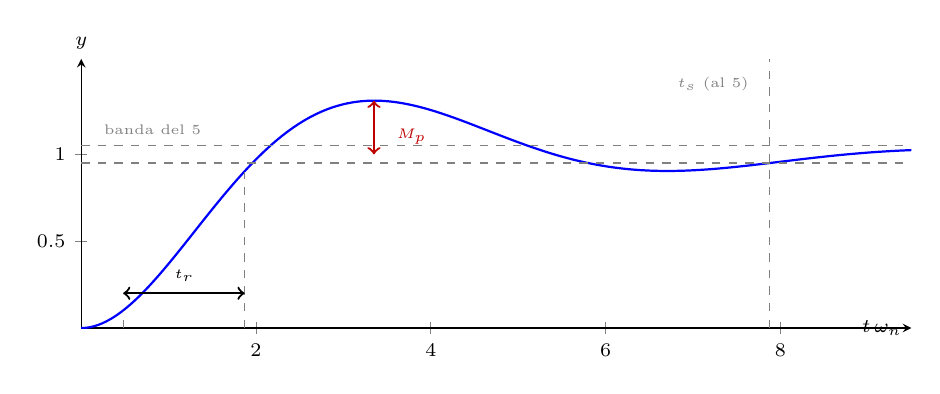
\begin{tikzpicture}
        \begin{axis}[
            width=\linewidth, height=5cm,
            xlabel={$t\,\omega_n$}, ylabel={$y$},
            xmin=0, xmax=9.5, ymin=0, ymax=1.55,
            axis lines=left, font=\scriptsize,
            xtick={2,4,6,8}, ytick={0.5,1},
            every axis y label/.style={at=(current axis.above origin),anchor=south},
            every axis x label/.style={at=(current axis.right of origin),anchor=east},
        ]
            \addplot[blue, thick, domain=0:9.5, samples=250]
                {1 - exp(-0.35*x)*(cos(deg(0.937*x)) + 0.374*sin(deg(0.937*x)))};
            % banda del 5 %
            \draw[dashed, gray] (axis cs:0,0.95) -- (axis cs:9.5,0.95);
            \draw[dashed, gray] (axis cs:0,1.05) -- (axis cs:9.5,1.05);
            \node[gray, font=\tiny, anchor=south west] at (axis cs:0.15,1.06) {banda del \SI{5}{\percent}};
            % sobreoscilación máxima
            \draw[<->, red!75!black, thick] (axis cs:3.35,1) -- (axis cs:3.35,1.309);
            \node[red!75!black, font=\tiny, anchor=west] at (axis cs:3.5,1.1) {$M_p$};
            % tiempo de subida (10 % a 90 %)
            \draw[dashed, gray] (axis cs:0.48,0) -- (axis cs:0.48,0.10);
            \draw[dashed, gray] (axis cs:1.87,0) -- (axis cs:1.87,0.90);
            \draw[<->, thick] (axis cs:0.48,0.2) -- (axis cs:1.87,0.2);
            \node[font=\tiny, anchor=south] at (axis cs:1.18,0.21) {$t_r$};
            % tiempo de establecimiento al 5 %
            \draw[dashed, gray] (axis cs:7.88,0) -- (axis cs:7.88,1.55);
            \node[gray, font=\tiny, anchor=north east] at (axis cs:7.75,1.5) {$t_s$ (al \SI{5}{\percent})};
        \end{axis}
    \end{tikzpicture}
    \caption[Prestaciones dinámicas medidas sobre la respuesta al escalón.]{Las prestaciones dinámicas que se especifican en una hoja de características, medidas sobre la respuesta al escalón de un sistema de segundo orden con $\zeta = 0{,}35$: el tiempo de subida $t_r$ (del \SI{10}{\percent} al \SI{90}{\percent}), la sobreoscilación máxima $M_p$ y el tiempo de establecimiento $t_s$ hasta entrar en la banda del \SI{5}{\percent}. El tiempo de subida y el de establecimiento fijan la rapidez; la sobreoscilación, el amortiguamiento.}\label{fig:prestaciones_dinamicas}
\end{marginfigure}

De los cuatro parámetros hay uno que merece una recomendación, porque aparece en todas las especificaciones y casi nunca se explica por qué: el amortiguamiento en torno a $\zeta \approx 0{,}7$ es el compromiso clásico, ya que da la respuesta más rápida sin sobreoscilación apreciable --menos de un \SI{5}{\percent}-- y un ancho de banda bien definido, con $f_c \approx \omega_n$. Es el valor que se busca cuando el ingeniero puede elegirlo --el amortiguamiento de un galvanómetro, la constante de tiempo de un filtro, el lazo de un circuito de disparo-- y el que conviene identificar en las especificaciones cuando viene impuesto.

\section{Límites de la Medida: Ruido y Rango Dinámico}\label{sec:limites_medida}

En esta sección se analizan los límites fundamentales de la medida, centrándonos en el ruido y el rango dinámico. Estos conceptos son cruciales para entender las limitaciones inherentes a cualquier sistema de medida y para diseñar sensores que puedan operar de manera efectiva dentro de estas limitaciones.

\subsection{El suelo de Ruido (\textit{Noise Floor})}\label{sec:noise_floor}
Una vez definidos los límites superiores (saturación), falta el límite inferior de la medida, que no es cero sino el \emph{suelo de ruido}: el nivel mínimo de señal que el sistema puede detectar por encima de su propio ruido --térmico, de disparo, de \textit{flicker}...--~\cite{ott1988noise}. Se expresa en las unidades de la magnitud medida, o en decibelios cuando conviene comparar rangos amplios. Su componente más predecible, el ruido térmico, se calcula como:
\begin{equation}\label{eq:noise_floor}
    N_f = \sqrt{4 k T R \Delta f}
\end{equation}
donde $k$ es la constante de Boltzmann, $T$ la temperatura absoluta, $R$ la resistencia del sistema y $\Delta f$ su ancho de banda: cuanto mayor sea cualquiera de los tres, mayor el ruido y peor la capacidad del sensor para detectar señales débiles.

\subsection{Ejemplo de Cálculo del Suelo de Ruido}\label{sec:ejemplo_suelo_ruido}
Con $R = \SI{1}{\kilo\ohm}$, $T = \SI{300}{\kelvin}$ y $\Delta f = \SI{1}{\kilo\hertz}$, la expresión~\eqref{eq:noise_floor} da:
\begin{equation}\label{eq:ejemplo_suelo_ruido}
    N_f = \sqrt{4 \cdot 1.38 \times 10^{-23} \cdot 300 \cdot 1000 \cdot 1000} \approx \SI{1.14}{\micro\volt}
\end{equation}
Ninguna señal por debajo de \SI{1.14}{\micro\volt} es fiable en este sistema. Bajar el suelo de ruido --componentes de bajo ruido, menor ancho de banda, un diseño de circuito cuidadoso-- es la única forma de detectar señales más débiles.

\subsection{Rango Dinámico}\label{sec:rango_dinamico}
El rango dinámico es la relación, en decibelios, entre la señal más fuerte que el sistema puede medir sin saturarse y la más débil que puede detectar por encima del suelo de ruido:
\begin{equation}\label{eq:rango_dinamico}
    R_D = 20 \log_{10} \left( \frac{S_{\max}}{N_f} \right)
\end{equation}
donde $S_{\max}$ es la señal máxima sin saturación y $N_f$ el suelo de ruido. Es una propiedad fija del sistema --no de la señal que se esté midiendo en cada momento-- y define su capacidad para medir simultáneamente señales muy grandes y muy pequeñas.\marginnote{\textbf{Importancia del Rango Dinámico:} Un micrófono con rango dinámico amplio captura tanto un susurro como un grito sin distorsión ni pérdida de información; de ahí que el rango dinámico se exprese en decibelios, que comprimen esas diferencias de varios órdenes de magnitud a una escala manejable.}

\subsection{Ejemplo de Cálculo del Rango Dinámico}
Con $N_f = \SI{1}{\micro\volt}$ y $S_{\max} = \SI{1}{\volt}$:
\begin{equation}
    R_D = 20 \log_{10} \left( \frac{1}{1 \times 10^{-6}} \right) = 20 \log_{10} (1000000) = \SI{60}{\decibel}
\end{equation}
Si el suelo de ruido sube a $N_f = \SI{10}{\micro\volt}$, el rango dinámico cae a:
\begin{equation}
    R_D = 20 \log_{10} \left( \frac{1}{10 \times 10^{-6}} \right) = 20 \log_{10} (100000) = \SI{40}{\decibel}
\end{equation}
Diez veces más ruido cuesta \SI{20}{\decibel} de rango: al ser una escala logarítmica, reducir el suelo de ruido a la mitad no duplica el rango dinámico utilizable.

\subsection{Relación Señal a Ruido (SNR)}\label{sec:snr}
La relación señal a ruido (SNR) compara, también en decibelios, el nivel de una señal concreta con el suelo de ruido del sistema:
\begin{equation}
    SNR = 20 \log_{10} \left( \frac{S}{N_f} \right)
\end{equation}
donde $S$ es el nivel de la señal que se desea medir y $N_f$ el suelo de ruido. A diferencia del rango dinámico --fijo para el sistema--, el SNR depende de la señal: cae a medida que esta se acerca al suelo de ruido, y con ella la fiabilidad de la medida.

\subsection{Ejemplo de Cálculo de la Relación Señal a Ruido (SNR)}\label{sec:ejemplo_snr}

Con $N_f = \SI{1}{\micro\volt}$ y $S = \SI{100}{\micro\volt}$:
\begin{equation}
    SNR = 20 \log_{10} \left( \frac{100 \times 10^{-6}}{1 \times 10^{-6}} \right) = 20 \log_{10} (100) = \SI{40}{\decibel}
\end{equation}
Si la señal cae a $S = \SI{10}{\micro\volt}$ --diez veces más débil--, el SNR baja a:
\begin{equation}
    SNR = 20 \log_{10} \left( \frac{10 \times 10^{-6}}{1 \times 10^{-6}} \right) = 20 \log_{10} (10) = \SI{20}{\decibel}
\end{equation}
El mismo suelo de ruido da lecturas mucho menos fiables cuando la señal es pequeña: es justo lo que distingue al SNR, que varía con la señal, del rango dinámico, que es fijo para el sistema.

Como se observa en la Figura~\ref{fig:noise_floor}, el diseño de un sistema de instrumentación es una lucha constante entre dos límites físicos. Por arriba, la Saturación limita la amplitud máxima que los amplificadores o el ADC pueden procesar sin distorsión. Por abajo, el Suelo de Ruido ($N_f$) establece el umbral mínimo de detectabilidad. La distancia total entre estos dos límites se conoce como Rango Dinámico (DR) y define la versatilidad del instrumento. Por el contrario, la Relación Señal-Ruido (SNR) es un parámetro operativo: cuanto más pequeña sea la señal de entrada, más cerca estará del suelo de ruido y menor será su SNR, lo que se traduce en una mayor incertidumbre en la medida.

\begin{marginfigure}
    \centering
    \shorthandoff{>}
    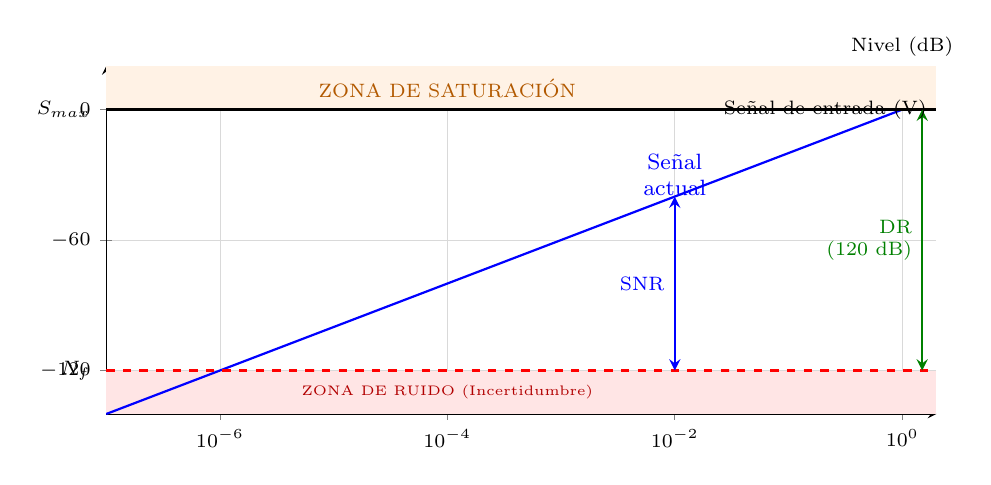
\begin{tikzpicture}
        \begin{axis}[
            width=\linewidth, height=6cm,
            xlabel={Señal de entrada (V)}, 
            ylabel={Nivel (dB)},
            xmode=log, % Escala logarítmica en X para ver décadas de voltaje
            xmin=1e-7, xmax=2,
            ymin=-140, ymax=20,
            axis lines=left,
            grid=both,
            grid style={line width=.1pt, draw=gray!10},
            major grid style={line width=.2pt,draw=gray!30},
            font=\scriptsize,
            xtick={1e-6, 1e-4, 1e-2, 1},
            ytick={-120, -60, 0},
            extra y ticks={-120, 0},
            extra y tick labels={$N_f$, $S_{max}$},
            every axis y label/.style={at=(current axis.above origin), anchor=south},
            every axis x label/.style={at=(current axis.right of origin), anchor=east},
        ]
            % 1. ZONA DE RUIDO (Sombreado)
            \fill[red!10] (axis cs:1e-7,-140) rectangle (axis cs:2,-120);
            \node[red!70!black, font=\tiny] at (axis cs:1e-4,-130) {ZONA DE RUIDO (Incertidumbre)};

            % 2. ZONA DE SATURACIÓN (Sombreado)
            \fill[orange!10] (axis cs:1e-7,0) rectangle (axis cs:2,20);
            \node[orange!70!black] at (axis cs:1e-4,10) {ZONA DE SATURACIÓN};

            % 3. CURVA DE SEÑAL
            \addplot[thick, blue, domain=1e-7:1, samples=100] {20*log10(x)};
            
            % 4. SUELO DE RUIDO (Línea horizontal)
            \addplot[thick, red, dashed, domain=1e-7:2] {-120};

            % 5. SEÑAL MÁXIMA (Línea horizontal)
            \addplot[thick, black, domain=1e-7:2] {0};

            % 6. ANOTACIÓN RANGO DINÁMICO (DR)
            \draw[<->, >=stealth, green!50!black, thick] (axis cs:1.5,-120) -- (axis cs:1.5,0) 
                node[midway, left, align=right] {DR\\(120 dB)};

            % 7. ANOTACIÓN SNR (en un punto concreto)
            \draw[<->, >=stealth, blue, thick] (axis cs:1e-2,-120) -- (axis cs:1e-2,-40) 
                node[midway, left] {SNR};
                
            \node[blue, align=center, font=\footnotesize] at (axis cs:1e-2, -30) {Señal\\actual};

        \end{axis}    
    \end{tikzpicture}        
    \caption[Diagrama de niveles de un sistema de medida.]{Diagrama de niveles de un sistema de medida. El \emph{Suelo de Ruido} ($N_f$) marca el límite inferior de detección, mientras que el nivel de \emph{Saturación} marca el límite superior. El \emph{Rango Dinámico} es una propiedad fija del sistema (\SI{120}{\decibel} en este ejemplo), mientras que la \emph{SNR} varía según la magnitud de la señal actual.}\label{fig:noise_floor}    
\end{marginfigure}

% \subsection{Resolución Real vs. Resolución Nominal}\label{sec:resolucion_real_vs_nominal}

% Es importante comprender que la resolución real de un sistema no es la que indica el número de bits del convertidor analógico a digital (ADC) o resolución nominal, sino la que impone el ruido. Si el ruido cuadrático médio o \textit{Root Mean Square} (RMS) es menor que el paso de cuantificación ($\Delta$), la resolución del sistema será la nominal y los bits menos significativos contendrán información sistemática. En cambio, si el RMS es mayor que el paso de cuantificación ($\Delta$), la resolución real del sistema estará degradada, sera inferior a la resolución nominal y los bits menos significativos solo contendrán información aleatoria.

% \begin{marginfigure}
%     \centering
%     \shorthandoff{>}
%     \begin{tikzpicture}
%         \begin{axis}[            
%             width=\linewidth, height=4.5cm,
%             xlabel={$t$}, ylabel={$y(t)$},
%             every axis y label/.style={at=(current axis.above origin),anchor=south},
%             every axis x label/.style={at=(current axis.right of origin),anchor=west},
%             axis lines=left,
%             grid=both,
%             grid style={line width=.1pt,draw=gray!10},
%             major grid style={line width=.2pt,draw=gray!30},
%             font=\scriptsize,
%             xtick={0, 1, 2, 3, 4, 5},
%             ytick={0, 0.5, 1},
%             legend style={at={(1,0.1)}, anchor=south east, font=\tiny, cells={anchor=west}}
%         ]
%             % 1. SEÑAL REAL (con ruido)
%             \addplot[thick, blue, domain=0:5, samples=200] {0.5 + 0.5*sin(deg(2*pi*0.5*x)) + 0.1*rand};
%             \addlegendentry{Señal con ruido}

%             % 2. SEÑAL NOMINAL (sin ruido)
%             \addplot[thick, red, domain=0:5, samples=200] {0.5 + 0.5*sin(deg(2*pi*0.5*x))};
%             \addlegendentry{Señal nominal}

%             % 3. PASO DE CUANTIFICACIÓN (Línea horizontal)
%             \addplot[thick, black, domain=0:5] {0.25};
%             \addlegendentry{Paso de cuantificación ($\Delta$)}

%             % 4. RESOLUCIÓN REAL            
%             \addplot[thick, green, domain=0:5, samples=200] {0.5 + 0.5*sin(deg(2*pi*0.5*x)) + 0.1*rand};
%             \addplot[thick, green, domain=0:5, samples=200] {0.5 + 0.5*sin(deg(2*pi*0.5*x))};
%             \addplot[thick, green, domain=0:5] {0.25};
%             \addlegendentry{Resolución real}

%             % 5. RESOLUCIÓN NOMINAL (Línea horizontal)
%             \addplot[thick, orange, domain=0:5] {0.0625};
%             \addlegendentry{Resolución nominal (4 bits)}
%         \end{axis}    
%     \end{tikzpicture}    
%     \caption{Resolución real vs. resolución nominal.}\label{fig:resolucion_real_vs_nominal}    
% \end{marginfigure}


\subsection{Resolución Nominal frente a Resolución Real}\label{sec:resolucion_real_vs_nominal}

En un sistema de medida digital, es fundamental distinguir entre el límite teórico impuesto por el hardware y el límite práctico impuesto por la física del ruido. La \emph{Resolución Nominal } viene determinada por el diseño del convertidor analógico a digital (ADC). Si el rango de entrada es $FS$ (\textit{Full Scale}) y el convertidor tiene $n$ bits, el paso de cuantificación $\Delta$ es:
    \begin{equation}
        \Delta = \frac{FS}{2^n}
    \end{equation}
    Este representa el \emph{peldaño} mínimo o \emph{paso de cuantificación} del sistema en ausencia total de ruido. La \emph{Resolución Real o Efectiva} es la resolución que el sistema puede alcanzar en la práctica. Depende de la relación entre el ruido cuadrático medio (\textit{Root Mean Square}, RMS) presente en la señal, $V_{n,RMS}$, y el paso de cuantificación $\Delta$.\marginnote{\textbf{Ruido \emph{pico a pico}:} Para que una medida sea estable en un display, el ruido pico a pico ($V_{pp}$) debe ser menor que $\Delta$. En una distribución gaussiana, se estima que $V_{pp} \approx 6.6 \cdot V_{n,RMS}$. Si $V_{pp} > \Delta$, los bits menos significativos oscilarán aleatoriamente, un fenómeno conocido como \textit{flicker} o parpadeo.} La variable $V_{n,RMS}$ representa el valor eficaz del ruido en la medida del cuantificador. En general, $V_{n,RMS}$ puede ser calculada con la siguiente fórmula:
    \begin{equation}
        V_{n,RMS} = \sqrt{4 k T R \Delta f}
    \end{equation}
    donde $k$ es la constante de Boltzmann, $T$ es la temperatura ambiente, $R$ es la resistencia del convertidor (o más exactamente la resistencia del sistema o resistencia equivalente de entrada) y $\Delta f$ es el ancho de banda del sistema. El ruido suelo o \textit{noise floor} es precisamente el valor de $V_{n,RMS}$, que representa el nivel mínimo de señal que el sistema puede detectar por encima del ruido inherente. Sólo una última aclaración, la ecuación del ruido cuadrático medio,  $V_{n,RMS}$, se basa en el modelo de ruido térmico (o de Johnson-Nyquist), pero en la práctica, el ruido total del sistema puede incluir otras fuentes de ruido, como el ruido de disparo, el ruido de flicker, entre otros. Por lo tanto, el valor real de $V_{n,RMS}$ puede ser mayor que el calculado solo con el ruido térmico, dependiendo de las características específicas del sistema y las condiciones de operación.

El comportamiento del sistema se puede clasificar en dos tipos de regímenes:     
\begin{enumerate}
    \item \emph{Sistema limitado por cuantificación} ($V_{n,RMS} \ll \Delta$): El ruido es tan bajo que queda \emph{escondido} dentro de un escalón de cuantificación. En este caso, la resolución real coincide con la nominal. Los bits menos significativos (\textit{Least Significant Bits}, LSB) son estables y contienen información útil de la magnitud física.
    \item \emph{Sistema limitado por ruido} ($V_{n,RMS} > \Delta$): El nivel de ruido es superior al escalón de cuantificación. La resolución real se degrada y el número efectivo de bits (ENOB, \emph{Effective Number of Bits}) es menor que el nominal ($n$). Los bits afectados por el ruido fluctúan aleatoriamente y no proporcionan información válida sobre la medida.
\end{enumerate}\marginnote{\textbf{Conclusión para el diseño:} No tiene sentido económico ni técnico utilizar un ADC de alta resolución (ej. 24 bits) si el ruido del sensor o de la etapa de acondicionamiento es muy elevado. El ingeniero debe equilibrar el suelo de ruido del hardware con la resolución del cuantificador.}

\section{Cómo se Lee una Hoja de Características}\label{sec:hoja_caracteristicas}

Todas las características anteriores acaban en una hoja de especificaciones, y leerla bien es tan importante como medir: dos instrumentos que anuncian la misma «exactitud del \SI{0.1}{\percent}» pueden comportarse de forma muy distinta según cómo esté referido ese número y en qué condiciones se haya medido. Conviene, por tanto, hacer tres preguntas a cada especificación.

\paragraph{¿Referida a la lectura o al fondo de escala?}
Una exactitud del \SI{0.1}{\percent} referida al fondo de escala es un error absoluto constante --siempre el mismo número de milivoltios--, mientras que referida a la lectura es proporcional al valor medido. La diferencia se aprecia al trabajar cerca del origen del rango, donde el error referido al fondo de escala se dispara en términos relativos:
\begin{equation}\label{eq:error_fs_lectura}
    e_{lectura} = e_{FS}\cdot\frac{\text{fondo de escala}}{\text{lectura}}
\end{equation}
de modo que un instrumento del \SI{0.1}{\percent} del fondo de escala empleado a una décima parte del rango se equivoca en un \SI{1}{\percent} de lo que indica. Por eso los multímetros de laboratorio especifican siempre dos términos: uno proporcional a la lectura y otro absoluto, con el que se cubren la deriva del cero y la resolución.

\paragraph{¿En qué condiciones?}
Toda especificación va referida a unas condiciones ambiente --habitualmente \SI{23}{\celsius} con una tolerancia de $\pm$\SI{5}{\celsius}-- y a una alimentación dadas. Fuera de ellas hay que añadir los coeficientes de las \emph{magnitudes de influencia}: la deriva térmica, en unidades por grado, y la sensibilidad a la tensión de alimentación. Ese término es el que arruina muchas medidas de campo y el que obliga a estabilizar la temperatura de una referencia o de un patrón (Capítulos~\ref{cap:metrologia} y~\ref{cap:ruido}).

\paragraph{¿Garantizada o típica?}
Un valor \emph{típico} es el que se obtiene en la mayoría de las unidades; un valor \emph{garantizado} o de peor caso es el que ninguna debe superar, y es el único que sirve para elaborar un presupuesto de errores como el de la Sección~\ref{sec:presupuesto_global}. La misma lógica se aplica a la estabilidad: una exactitud del \SI{0.01}{\percent} en veinticuatro horas puede degradarse a diez veces más en un año si el instrumento no se recalibra, de modo que el intervalo de calibración forma parte de la especificación tanto como el propio número.

La Tabla~\ref{tab:caracteristicas_medida} recoge, como resumen del capítulo, las características estudiadas, su símbolo y la forma habitual en que se especifican.

\begin{table}[ht]
    \centering
    \small
    \setlength{\tabcolsep}{3pt}
    \forcerectofloat % la tabla cae en página impar (recto); sin forzar, el caption sale al lado contrario
    \begin{tabularx}{\linewidth}{@{} L{0.24\linewidth} >{\centering\arraybackslash}X >{\centering\arraybackslash}X @{}}
        \toprule
        \textbf{Característica} & \textbf{Se especifica como} & \textbf{Dónde se estudia} \\
        \midrule
        Sensibilidad ($S$) & Pendiente de la curva de calibración: unidades de salida por unidad de entrada & Sección~\ref{sec:caract_estaticas} \\
        Linealidad & Desviación máxima respecto a la recta de referencia, en \% del fondo de escala & Sección~\ref{sec:error_no_linealidad} \\
        Histéresis y repetibilidad & Diferencia máxima entre las ramas y dispersión con entrada constante, en \% del fondo de escala & Sección~\ref{sec:histeresis_repetibilidad} \\
        Error de cero y de span ($e_0$, $\epsilon_s$) & El de cero en unidades absolutas; el de span en \% de la lectura & Sección~\ref{sub:error_cero_span} \\
        Resolución ($\Delta$) & Escalón más pequeño discernible, nominal y efectivo & Sección~\ref{sec:resolucion_real_vs_nominal} \\
        Efecto de carga & Error por la impedancia de entrada, en \% de la lectura & Sección~\ref{sub:efecto_carga_general} \\
        Prestaciones dinámicas ($t_r$, $M_p$, $t_s$, $f_c$) & Tiempos medidos sobre la respuesta al escalón y frecuencia de corte & Sección~\ref{sub:prestaciones_dinamicas} \\
        Suelo de ruido y rango dinámico ($N_f$, $DR$) & Nivel mínimo detectable y cociente con el máximo, en decibelios & Sección~\ref{sec:limites_medida} \\
        Deriva térmica & Unidades por grado centígrado, fuera de las condiciones de referencia & Sección~\ref{sec:hoja_caracteristicas} \\
        \bottomrule
    \end{tabularx}
    \caption[Características de un sistema de medida y su forma de especificarlas.]{Resumen de las características de un sistema de medida, la forma habitual de especificarlas y la sección donde se estudian. Es la lista que hay que recorrer al leer una hoja de características y la misma que se necesita, término a término, para elaborar un presupuesto de errores.\protect\label{tab:caracteristicas_medida}}
\end{table}

\section{Resumen}\label{sec:resumen_caracteristicas}

En este capítulo se ha fijado el vocabulario con el que se describe un sistema de medida, que es el que aparece después en las hojas de características, en los pliegos de condiciones y en los presupuestos de error del resto del libro:

\begin{itemize}
    \item \emph{Características estáticas} (Sección~\ref{sec:caract_estaticas}): la curva de calibración y su sensibilidad, la linealidad y la recta de referencia, la histéresis, la repetibilidad y la reproducibilidad, el rango y la saturación, y los dos defectos de la recta --error de cero y error de span (Figura~\ref{fig:errores_cero_span})--, junto con el efecto de carga, que aparece siempre que dos etapas con impedancias comparables se conectan entre sí.
    \item \emph{Características dinámicas} (Sección~\ref{sec:caract_dinamicas}): la respuesta al escalón de los sistemas de orden cero, primero y segundo, con la constante de tiempo, la frecuencia natural y el amortiguamiento como parámetros; y las prestaciones con las que se especifican --tiempo de subida, sobreoscilación máxima, tiempo de establecimiento y ancho de banda (Figura~\ref{fig:prestaciones_dinamicas})--, con $\zeta \approx 0{,}7$ como el compromiso recomendado entre rapidez y estabilidad.
    \item \emph{Límites de la medida} (Sección~\ref{sec:limites_medida}): el suelo de ruido, el rango dinámico y la relación señal-ruido, junto con la diferencia entre resolución nominal y resolución real (Figura~\ref{fig:noise_floor}), que es lo que fija hasta dónde se puede medir y no solo qué se puede medir.
    \item \emph{Cómo se lee una hoja de características} (Sección~\ref{sec:hoja_caracteristicas}): si la especificación está referida a la lectura o al fondo de escala (ecuación~\eqref{eq:error_fs_lectura}), en qué condiciones de referencia se ha medido, si el valor es típico o garantizado y qué magnitudes de influencia hay que añadir en cada caso; la Tabla~\ref{tab:caracteristicas_medida} reúne todas las características del capítulo con su forma de especificarlas.
\end{itemize}

\marginnote{\textbf{Conclusión:} ninguna de las características de este capítulo se puede mejorar más adelante. La exactitud de un sistema de medida queda fijada cuando se eligen el sensor y su acondicionamiento, y lo que hace el resto del libro es conservarla: digitalizarla sin degradarla (Capítulo~\ref{cap:daq}), protegerla del entorno (Capítulo~\ref{cap:ruido}) y transmitirla sin perderla (Capítulo~\ref{cap:buses}).}
